\documentclass[lettersize,journal]{IEEEtran}

% MY PACKAGES ===================================
\usepackage{epsfig}
\usepackage{lipsum}  
\usepackage{kotex}
% \usepackage{natbib}
\usepackage{cite}
\usepackage{amssymb}
\usepackage{xcolor}
\usepackage{enumitem}
\newlist{steps}{enumerate}{1}
\setlist[steps, 1]{label = Step \arabic*: }
\usepackage{hyperref}
\hypersetup{
    linkbordercolor=blue,
    filebordercolor=red,
    citebordercolor = green,      
    urlbordercolor=red,
    %
    % colorlinks=true,
    % linkcolor=blue,
    % filecolor=blue,
    % citecolor = blue,      
    % urlcolor=cyan,
 }
 \usepackage{algorithm}
 \usepackage{svg}

% MY PACKAGES ===================================

\usepackage{amsmath,amsfonts}
\usepackage{algorithmic}
\usepackage{array}
% \usepackage[caption=false,font=normalsize,labelfont=sf,textfont=sf]{subfig}
\usepackage{subfig}
\usepackage{textcomp}
\usepackage{stfloats}
\usepackage{url}
\usepackage{verbatim}
\usepackage{graphicx}
\hyphenation{op-tical net-works semi-conduc-tor IEEE-Xplore}
\def\BibTeX{{\rm B\kern-.05em{\sc i\kern-.025em b}\kern-.08em
    T\kern-.1667em\lower.7ex\hbox{E}\kern-.125emX}}
\usepackage{balance}

% MY PACKAGES ===================================
% \let\proof\relax
% \let\endproof\relax
\usepackage{amsthm}
\newtheorem{remark}{Remark}
\newtheorem{assum}{Assumption}
\newtheorem{lem}{Lemma}
\newtheorem{theorem}{Theorem}

% MY PACKAGES ===================================

\begin{document}
\title{
% \color{red}
Constrained Optimization-Based Neuro-Adaptive Control (CoNAC) for Uncertain Euler Lagrangian Systems With Input Saturation
% \color{black}
}
\author{Myeongseok Ryu, Donghwa Hong, and Kyunghwan Choi,~\IEEEmembership{Member,~IEEE}
\thanks{Manuscript created Month, 2024; This work was supported by Korea Research Institute for Defense Technology planning and advancement (KRIT) grant funded by Korea government DAPA (Defense Acquisition Program Administration) (No. KRIT-CT-22-087, Synthetic Battlefield Environment based Integrated Combat Training Platform). \it{(Corresponding author: Kyunghwan Choi)}}}

\markboth{IEEE TRANSACTIONS ON NEURAL NETWORKS AND LEARNING SYSTEMS,
~Vol.~00, No.~0, Month~2024
}%
{How to Use the IEEEtran \LaTeX \ Templates}

\maketitle

\begin{abstract}
    In this paper, a constrained optimization-based neuro-adaptive controller (CoNAC) is proposed for uncertain Euler-Lagrange systems in the presence of the nonlinear physical-input saturation. 
    The controller consists of a back-stepping controller (BSC)-based reference generator, a deep neural network (DNN), and a weight optimizer for the DNN.
    The weight optimizer is developed to minimize the Lagrangian function with respect to the DNN weights and the Lagrange multipliers of the constraints.
    In the steady-state, the proposed controller satisfies the Karush-Kuhn-Tucker (KKT) conditions.
    The stability of the proposed controller is analyzed using Lyapunov theory and it ensures that the tracking error and the estimation error of the DNN weights are bounded. 
    The performance of the proposed controller is compared with three selected controllers through numerical simulations. 
    The simulation results demonstrate that the proposed controller can regulate the tracking error with constraint satisfaction.
\end{abstract}

\begin{IEEEkeywords}
Neuro-adaptive control, constrained optimization, deep neural network, Euler-Lagrange system, input saturation.
\end{IEEEkeywords}

%  SECTION INTRODUCTION ===================================
\section{Introduction}

\subsection{Background}

\IEEEPARstart{T}{ime} varying and uncertain systems are common in various engineering applications, such as aerospace, robotics, and automotive systems. 
Due to the presence of uncertainty, the control performance index of the controller may degrade, resulting in the system's instability.
To compensate the uncertainty, adaptive control approaches have been widely used \cite{RN4}, \cite{RN2}.
The conventional adaptive control approaches generally estimate certain unknown parameters in the system or the controller.

More recently, the neuro-adaptive control approaches using the approximation theory \cite{RN1} have been introduced to approximate the unknown dynamics of the system or the whole controller directly, using neural networks (NNs).
It is well-known that the NNs have the universal approximation property which claims that they can approximate a smooth function in a compact set with a small approximation error.
However, using the NNs in the controller, the control input saturation can occur, since the boundedness of the ranges of the NNs is not proved.

The control input also can be saturated in many industry control systems, since the actuators generally have the limitations of their feasible amplitudes of control inputs, due to the physical characteristics or safety considerations \cite{RN18}.
The controllers without the consideration of the saturation may have a lower performance index or destroy the stability of the system.
Therefore, the saturation of the control input is required to be addressed in the neuro-adaptive controller design.

\subsection{Literature Review}

Due to the simplicity of the mathematical expression of the architecture, single-hidden layer NNs (SLNs) \cite{RN29} and Radial Basis Function (RBF) NNs \cite{RN26} are widely used in the neuro-adaptive controller design.
% SLN, RBF refs here
The architecture of the SLNs consists of the input layer, the single hidden layer, and the output layer, and the activation function of the hidden layer is generally the sigmoid function or the hyperbolic tangent function \cite{RN44, RN56, RN54, RN3, RN41}.
On the other hand, the RBF NNs use the RBFs as the activation function \cite{RN10, RN34, RN37, RN31, RN7, RN11}.

% how NNs works
These NNs are usually used to synthesize NNs and conventional controllers.
For a feedback-linearization controller and the backstepping (BSC) controller, the NNs are used to approximate and cancel the unknown dynamics of the system in \cite{RN44, RN56} and \cite{RN10, RN31, RN57}, respectively. 
To use these controllers, the singularity problems should be addressed since the approximated control coefficient function can be closed to zero (i.e., the approximated control coefficient function is inversed in the controller).
To reject the disturbance, the NN is used in the sliding mode controller \cite{RN7}.
In \cite{RN34} and \cite{RN37}, the NNs are combined with impedance control and admittance control, respectively, for the manipulator control.
By compensating the unknown system dynamics, the controllers can improve the tracking performances even with the poorly tuned control parameters.
% Direct Approx
A few studies used the NNs to directly approximate the whole desired controller \cite{RN54, RN3}.
Since the controllers are directly approximated, the singularity problem can be avoided.

% how the adapation law derived
Most of the existing literature derives the adaptation laws of the weights based on the Lyapunov analysis and the boundedness or the convergence of the tracking error and the estimation error of the weights are guaranteed.
On the other hand, the optimization-based adaption law with respect to the quadratic tracking error objective function using the gradient descent method is introduced by Esfandiari \textit{et al.} in \cite{RN56, RN54, RN3}.
% concludes
Despite the simple structure of the NNs, the existing works have shown that the neuro-adaptive controllers can approximate the unknown dynamics of the system and the controller effectively with improved performance.

However, as reported in \cite{RN25}, Deep NNs (DNNs) are exponentially more expressive than shallow NNs with the same total number of weights.
It means that the DNNs are practically more effective in approximation since low computational costs are required.
In this manner, the neuro-based adaptive controller with DNN is introduced \cite{RN16}. 
Furthermore, the variations of the DNN are also utilized in the adaptive controller: 
in \cite{RN14}, the Long short-term memory (LSTM) is used to capture the time-varying system dynamics; 
\cite{RN15} introduced the Physics-informed NN and LSTM in the controller, to leverage the prior knowledge of the physical system features.
The adaptation laws of these studies are also derived from the Lyapunov analysis with the boundedness of the tracking error and the estimation error of the weights guarantee.

The common issue in the stability analysis of the neuro-adaptive control is the boundedness of the weights in the NNs.
In \cite{RN16, RN14, RN11}, the projection operator is used to make the norms of the weights be lower than some positive constants.
The positive constants are usually selected as large as possible since the global optimal point can not be analyzed.
\color{red}
In other literature, using the $\epsilon$-modification method to make the invariance set of the weights [] [].
\color{black}
Using $\epsilon$-modification, the stable function appears in the adaptation law. % 혹시 이해가 되시나요? stable하게 하는 함수가 생긴다는 걸 말하고 싶은데...
However, these studies have no theoretical analysis of the optimality of the adapted weights.

The other common issue is that the outputs of the NNs are not predictable
It means the NNs in the controllers can produce the large control input resulting in the control input saturation.
Besides, if the neuro-adaptive controllers are based on the conventional controllers that cancel the system dynamics, the control input may be excessively large.
It is because the conventional controllers may try to cancel the stabilizing system dynamics unnecessarily.
Since there are control input limitations due to the physical characteristics of the system, the saturation should be tackled.
Considering the control input saturation, the auxiliary systems are generally used to mitigate the effect of the saturation of the control input.
In \cite{RN55, RN56, RN54, RN3}, the auxiliary states are generated when the saturation occurs and added to the errors in the adaptation law.
Then the weights are also adapted to reduce the saturation by regulating the generated auxiliary states.
On the other hand,
the auxiliary states can be used as the feedback term in the control law to compensate the saturation \cite{RN34, RN38, RN37, RN36}.
% The fixed-time \cite{RN57}
% the fractional exponential powers into the existing asymptotic convergent auxiliary system
% An adaptive auxiliary system is constructed to mitigate the effect of actuator saturation. The designed auxiliary system is capable of achieving the same fixed-time convergence rate as the backstepping controller.
In \cite{RN41}, the NN is employed to approximate the desired saturation compensator's control input.
These existing studies only consider the saturation of each control input.
\color{red} However, the nonlinear control input saturation functions appear in many physical systems in robotics [], motor systems [] [], and so on. \color{black}

The presented issues including the boundedness of the weights and the control saturation, can be transformed to the constraints in the adaptation process.
To adapt the weights to minimize the objective function with the constraints satisfaction, the constrained optimization theory based approach can be utilized.
The constrained optimization theory theoretically defines the optimality and presents the methods to obtain the solution numerically \cite{RN22}.
In some literature, constrained optimization methods such as the Augmented Lagrangian method (ALM) \cite{RN59} and the Alternating direction method of multipliers \cite{RN58, RN60} are used to train the NNs.
The imposed constraints in the literature are related to the architecture of the NNs to avoid the gradient vanishing issue of backpropagation.

\subsection{Contributions}

The main contributions of this study are listed as follows:
\begin{itemize}
    \item The nonlinear control saturation functions and the boundedness of the weights are handled by transforming them to the inequality constraints in the adaptation process.   
    The simulation demonstrated that the proposed controller improve the performance index while satisfying the constraints.
    \item The neuro-adaptive controller with DNN whose adaptation law is derived based on the constrained optimization theory is presented.
    By minimizing the Lagrangian function with respect to the weights and the Lagrange multipliers, they are available to reach the local optimal point which satisfies the KKT conditions.
    \item To calculate the gradient of the objective function which includes the error dynamics, the forward sensitivity method is used.
    By simulating the dynamics of the sensitivity of the weights to error, the exact gradient can be obtained.
\end{itemize}

\subsection{Organization}

The remainder of this paper is organized as follows:
Section \ref{sec: Problem Formulation} presents the target-constrained system and control objective.
Section \ref{sec:ctrl design} introduces the proposed controller and the architecture of DNN in the controller. 
In Section \ref{sec:adap_laws}, the optimizer of the weights in the DNN is developed.
Section \ref{sec:stability} examines the stability of the proposed controller.
A comparative study of the four selected controllers including the proposed controller is reported in Section \ref{sec:sim}.
Finally, Section \ref{sec:conclusion} concludes the paper by presenting a future work.
The presented appendices provide the candidates of the constraints, and the proof of the used Lemma in stability analysis.

%  SECTION PROBLEM FORMULATION ============================
\section{Problem Formulation}\label{sec: Problem Formulation}

\subsection{Notation}
In this study, the following notation is used.

\begin{itemize}
    \item $\otimes$ denotes the Kronecker product \cite{RN17}.
    \item $x_{(i)}$ denotes the $i\textsuperscript{th}$ element of vector $x$.    
    % \item $A_{(i,j)}$ is the $i\textsuperscript{th}$ row-$j\textsuperscript{th}$ column element of matrix $A$.
    \item $\text{row}_j(A)$ denotes the $j\textsuperscript{th}$ row of $A\in\mathbb{R}^{n\times m}$. 
    % \item $\text{col}_i(A)$ and $\text{row}_j(A)$ denote the $i\textsuperscript{th}$ column and $j\textsuperscript{th}$ row of $A\in\mathbb{R}^{n\times m}$, respectively.
    \item $\text{vec}(A)\triangleq [\text{row}_1(A^T)  ,\cdots,\text{row}_m(A^T)  ]^T   $ for $A\in\mathbb{R}^{n\times m}$.
    % \item $\text{vec}(A)\triangleq [\text{col}_1(A)^T  ,\cdots,\text{col}_m(A)^T  ]^T   $ for $A\in\mathbb{R}^{n\times m}$.
    \item $\lambda_\text{min}(A)$ denotes the minimum eigenvalue of $A\in\mathbb{R}^{n\times n}$.
\end{itemize}

\subsection{Model Dynamics and Control Objective}

Consider an uncertain Euler-Lagrange system modeled as
\begin{equation}
    M(q)\ddot q + C(q,\dot q)\dot q + G(q) + F(q) = h(\tau)
    \label{eq. system dynamics 1}
\end{equation}
where $q\in \mathbb{R}^n$ denotes the generalized coordinate; $\tau\in\mathbb{R}^n$ denotes the control input; $M(q)\in\mathbb{R}^{n\times n}$, $C(q,\dot q)\in\mathbb{R}^{n\times n}$, and $G(q)\in\mathbb{R}^{n}$ denote the unknown system function matrices; $F(q)\in\mathbb{R}^{n}$ denotes the external force; and $h(\cdot)$ denotes the smooth nonlinear control input saturation function whose gradient with respect to $\tau$ is also bounded, i.e., $\Vert\partial h/\partial \tau\Vert_F\in L_\infty$. 

The saturation function represents the physical limitations of the actuators.
Considering the physical limitations, physical-motivated constraints should be addressed in the controller design.
In Appendix \ref{sec:cstr candidates}, the candidates of the constraints are introduced.

Using user-designed nominal system matrices $M_0,C_0>0$ and $G_0$, \eqref{eq. system dynamics 1} can be reformulated as
\begin{equation}
    M_0\ddot q+C_0\dot q+G_0 = h(\tau) + f(q,\dot q,\ddot q)
    \label{eq. system dynamics 2}
\end{equation}
where $f(q,\dot q,\ddot q) \triangleq -\Delta M(q)\ddot q-\Delta C(q,\dot q)\dot q -\Delta G(q) -F(q)\in\mathbb{R}^n$ is the unknown lumped residual term with $\Delta M(q)\triangleq M(q)-M_0$, $\Delta C(q,\dot q)\triangleq C(q,\dot q)-C_0$, and $\Delta G(q)\triangleq G(q)-G_0$. 
The function $f$ acts like an external disturbance, resulting in poor performance index and instability.
Hence, an adaptive control approach is needed to improve the control performance.

In summary, the control objective is to develop a neuro-adaptive controller for $q$ to track the continuously differentiable desired trajectory $r_1(t): \mathbb{R} \to \mathbb{R}^n$ tackling the constraints.

%  SECTION CONTROLLER DESIGN ==============================
\section{Control Law Development}\label{sec:ctrl design}

The overall controller is presented in Fig.~\ref{fig: controller} consisting of:
Neuro-adaptive controller with BSC-based reference generator and DNN, and weight optimizer for the DNN.
To break down the original system into lower dimension subsystems, the BSC approach is utilized to design the controller \cite{RN38}, since \eqref{eq. system dynamics 1} is $2\textsuperscript{nd}$-order system.

\begin{figure*}[!t]
    \centering
    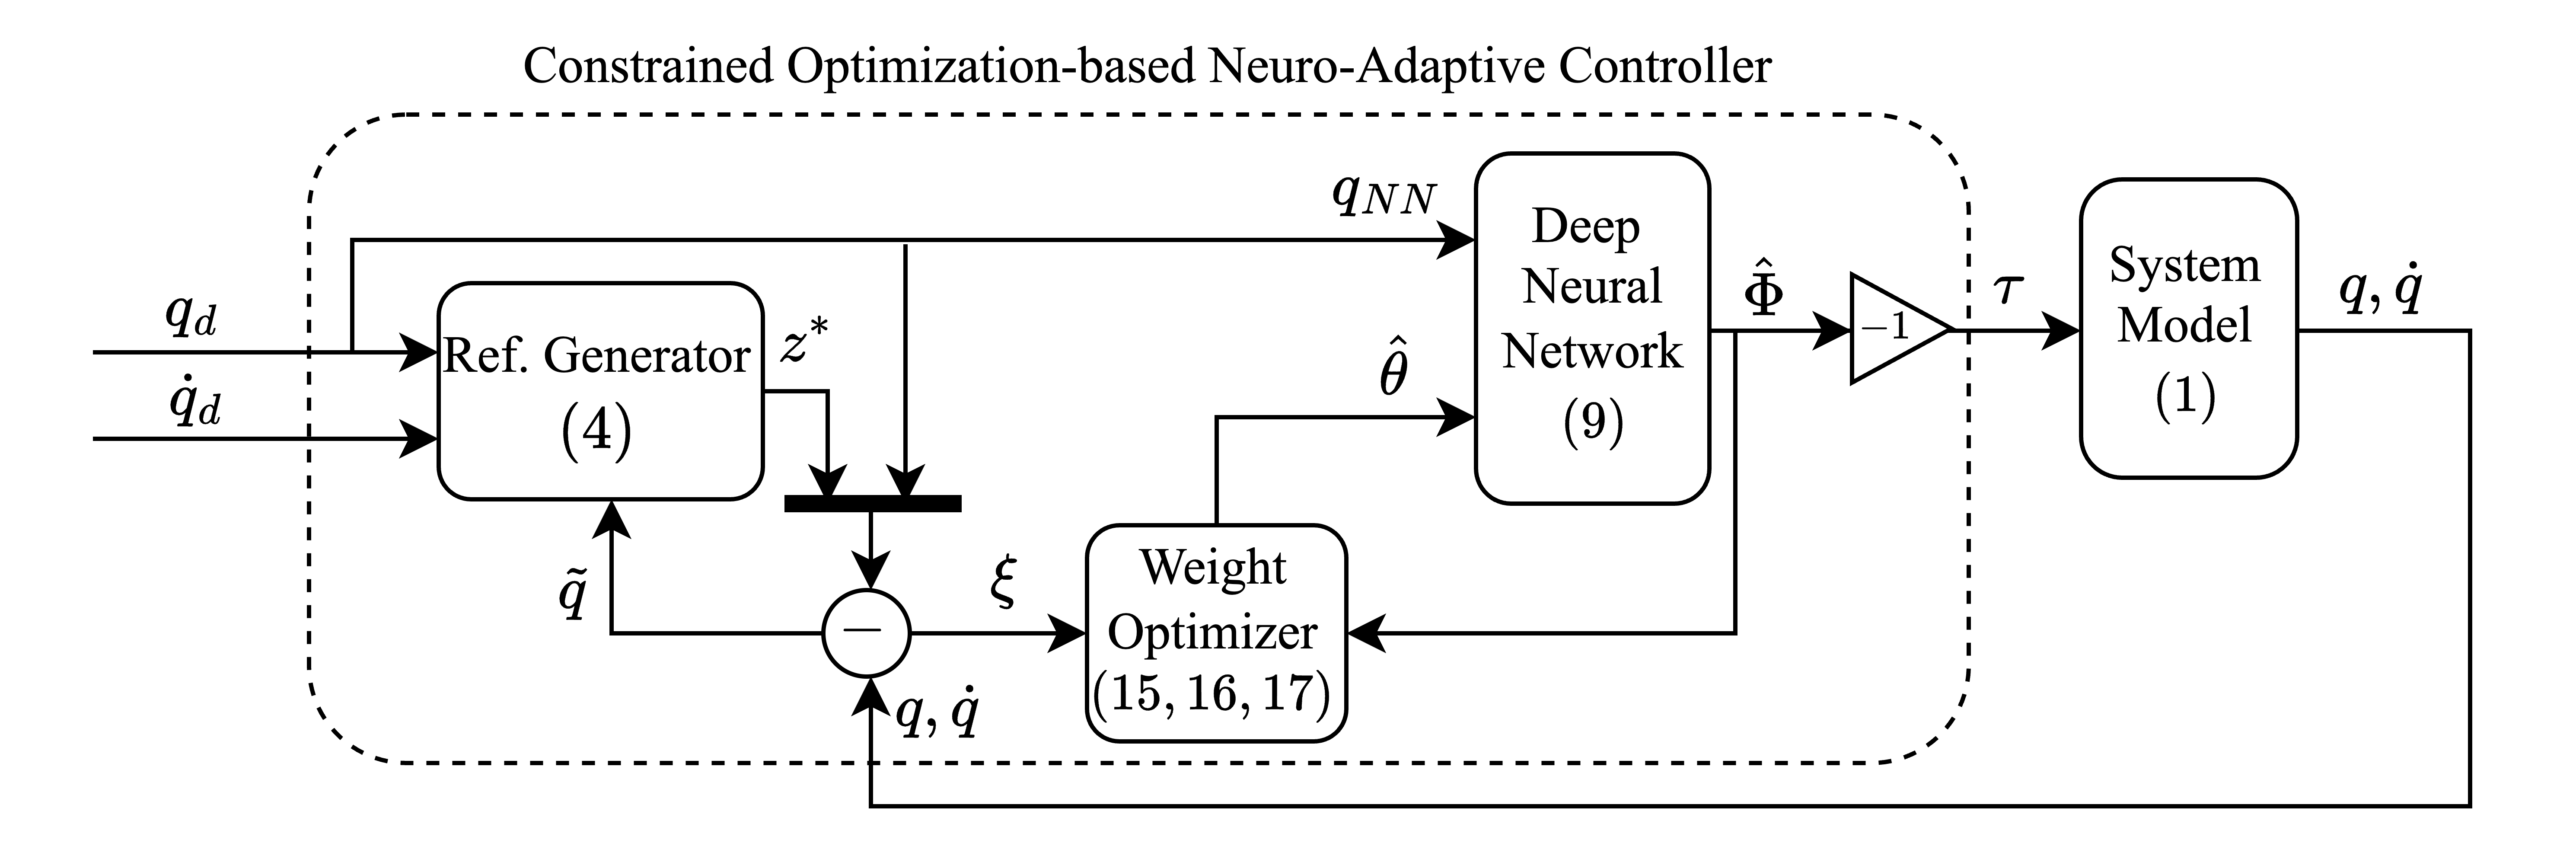
\includegraphics[width=0.7\linewidth]{Controller.drawio.png}
    % \includesvg[width=0.75\linewidth]{Controller.drawio.svg}
    \caption{Proposed Controller.}
    \label{fig: controller}
\end{figure*}

\subsection{Neuro-Adaptive Controller Design}

The system dynamics \eqref{eq. system dynamics 2} can be represented as
\begin{equation}
    \begin{aligned}
        \dot x_1 &= x_2,\\
        \dot x_2 &= -M_0^{-1} C_0 x_2-M_0^{-1} G_0+M_0^{-1} h(\tau) + M_0^{-1} f
    \end{aligned}
    \label{eq. x dynamics}
\end{equation}
where $x_1\triangleq q$ and $x_2\triangleq \dot q$.

Consider the Lyapunov function $V_{c1}\triangleq(1/2)e_1^T  e_1$, where $e_1\triangleq x_1-r_1$ denotes the tracking error of $x_1$. 
The desired trajectory of $x_2$ that ensures $\dot V_{c1}=e_1^T  (x_2-\dot r_1)<0$ is 
\begin{equation}
    r_2 \triangleq -k_1e_1 + \dot r_1
\end{equation}
with $k_1 \in\mathbb{R}_{>0}$. The tracking error of $x_2$ relative to the desired auxiliary trajectory $r_2$ is defined as
\begin{equation}
    e_2 \triangleq x_2 - r_2 = x_2 - (-k_1e_1 + \dot r_1).
    \label{eq. e2}
\end{equation}

Next, consider the Lyapunov function $V_{c2}\triangleq V_{c1} + (1/2) e_2^T  e_2$.
Its time derivative is
\begin{equation}
    \begin{aligned}
    \dot V_{c2} &=
    e_1^T  (-k_1e_1+e_2) +e_2^T  (-M_0^{-1} C _0x_2 -M_0^{-1} G_0\\
    &\quad
    +M_0^{-1}h(\tau)+M_0^{-1} f- \dot r_2)\\
    &= -k_1e_1^T  e_1 -k_2e_2^T  e_2 +e_2^T  (k_2e_2+e_1\\
    &\quad-M_0^{-1} C_0x_2 -M_0^{-1} G_0+M_0^{-1} h(\tau)+M_0^{-1} f- \dot r_2 )
    \end{aligned}
\end{equation}
with $k_2\in\mathbb{R}_{>0}$. 
The stabilizing     control input which does not address the control input saturation is defined as follows:
\begin{equation}
    \tau^* \triangleq-M_0\cdot (k_2e_2)+ 
    ( 
        -M_0e_1+C_0x_2+G_0-f+M_0 \dot r_2
    ).
    \label{eq. desired control}
\end{equation}
This control input ensures that the time derivative of the Lyapunov function is negative definite, as $\dot V_{c2} = -k_1e_1^T  e_1-k_2e_2^T  e_2<0$, if there is no control input saturation.
Note that, the actual $\tau^*$ can not be realized, since there is no information of $f$, which is unknown.

Let $\Phi\triangleq\Phi(q_N;\theta): \mathbb{R}^{l}\times\mathbb{R}^{\Xi}\to\mathbb{R}^{n}$ be the DNN where $q_N\in\mathbb{R}^{l}$ is a neural network input vector and $\theta\in\mathbb{R}^{\Xi}$ is a vectorized trainable weights.
The architecture of the $\Phi(q_N;\theta)$ will be defined in Section \ref{NN definition}.
According to the universal approximation theorem of DNNs \cite{RN33}, $\Phi(q_N;\theta)$ has the capability to approximate a nonlinear function $g(\cdot)$ with an ideal weight vector $\theta^*$ for a compact subset $\Omega_n\in\mathbb{R}^{l}$ to $\epsilon$-accuracy, such that $\sup_{q_N\in\Omega_n}\Vert \Phi(q_N;\theta^*) - g(\cdot) \Vert = \epsilon < \infty$.
Furthermore, the theorem states that the norm of the $\theta^*$ is bounded, i.e., $\Vert\theta^*\Vert\le \bar\theta<\infty$.
In this study, $\theta^*$ is defined as a local optimal point, not a global optimal point.
%within the compact subset $\Omega_\theta=\{\theta^* \ \vert\ \Vert\theta^*\Vert\le \bar\theta\}$, where $\bar\theta$ denotes the user-selected maximum norm of the weight, ensuring $\epsilon$-accuracy.

Using $\Phi(q_N;\theta)$, and the ideal and estimated weight vector the control inputs are approximated as follows:
\begin{equation}
    \tau^*\approx -
    (
        \Phi(q_N;\theta^*)+\epsilon
    )
    ,\quad 
    \tau \triangleq -\Phi(q_N;\hat\theta)
    \label{eq. approximated control}
\end{equation}
where $\hat\theta$ is the estimated vector of $\theta^*$.

Using \eqref{eq. x dynamics}, \eqref{eq. e2}, \eqref{eq. desired control}, \eqref{eq. approximated control}, the error dynamics can be obtained as
\begin{equation}
    \begin{aligned}
        \dot e_1 = & -k_1 e_1 + e_2 \\
        \dot e_2 = & -e_1 -k_2 e_2 + M_0^{-1} (\Phi^*-h(\hat\Phi)+\epsilon) 
    \end{aligned}
    \label{eq. error dynamics1}
\end{equation}
where $\Phi^*\triangleq \Phi(q_N;\theta^*)$ and $\hat\Phi\triangleq \Phi(q_N;\hat\theta)$.
The error dynamics \eqref{eq. error dynamics1} can be represented by a first-order system as 
\begin{equation}
    \dot\xi = A_\xi \xi + B_\xi (\Phi^*-h(\hat\Phi)+\epsilon)
    \label{eq. xi dynamics}
\end{equation}
where 
$\xi\triangleq[e_1^T  , e_2^T  ]^T  \in\mathbb{R}^{2n}$ denotes the augmented error
and
\begin{equation*}
    A_\xi \triangleq 
    \begin{bmatrix}
        -k_1 I_n &I_n\\-I_n& -k_2 I_n
    \end{bmatrix}
    ,\ 
    B_\xi \triangleq 
    \begin{bmatrix}
        0\\M_0^{-1}
    \end{bmatrix}.
\end{equation*}
Note that $A_\xi$ is a stable matrix and $\Vert B_\xi\Vert_F<\infty$.
% According to \eqref{eq. xi dynamics}, $\xi$ will be regulated as $\hat\theta \rightarrow \theta^*$.

\subsection{Deep Neural Network (DNN) Model}\label{NN definition}

The architecture of the DNN presented in \cite{RN16} is utilized in this study and is defined as follows:
\begin{equation}
    \Phi(q_N;\theta) \triangleq V_k^T  \phi_{k}(V_{k-1}^T   \cdots \phi_2(V_1^T   \phi_1(V_0^T   q_N))\cdots ))
    \label{eq. DNN structure 1}
\end{equation}
where $V_i\in\mathbb{R}^{(l_i+1)\times l_{i+1}}$ is the weight matrix of the $i\textsuperscript{th}$ layer; and $\phi_i: \mathbb{R}^{l_i}\to\mathbb{R}^{l_i+1}$ represents the activation function of the $i\textsuperscript{th}$ layer, which is defined by $\phi_i(x)=[\sigma(x_{(1)}),\sigma(x_{(2)}),\cdots, \sigma(x_{(l_{i})}), 1]^T$ with a nonlinear function $\sigma: \mathbb{R}\to\mathbb{R}$ and augmentation of $1$ to combine the bias terms in the weight matrices. Notice that the size of the output of $\Phi(\cdot)$ is the same as that of the control input $\tau$ (i.e., $l_{k+1}=n$).
For a better intuition, \eqref{eq. DNN structure 1} also can be represented recursively as 
\begin{equation*}
    \Phi_i \triangleq
    \begin{cases}
        V_i^T  \phi_i(\Phi_{i-1}), &i\in[1,\dots,k],\\
        V_0^T  q_N,&i=0,
    \end{cases}
    \label{eq. DNN structure 2}
\end{equation*}
where $\Phi_k = \Phi(q_N;\theta)$.

One of the widely used activation functions for large DNNs is the ReLU family \cite{RN27}, which effectively avoids the gradient vanishing problem during error backpropagation. In contrast, for control applications where relatively shallow DNNs are typically sufficient and the gradient vanishing issue is less severe, the sigmoid function or the hyperbolic tangent function can be used as activation functions. These functions simplify stability analysis due to their continuous differentiability and bounded outputs and gradients, satisfying $\Vert \phi_i(\cdot)\Vert < \infty, \Vert \nabla\phi_i(\cdot)\Vert_F < \infty$.
In this study, the hyperbolic tangent function $\tanh(\cdot)$ was selected as the activation function (i.e., $\sigma(\cdot) = \tanh(\cdot))$, which provides desirable boundedness with $\Vert\sigma(\cdot)\Vert<1, \Vert\nabla\sigma(\cdot)\Vert< 1$.

For simplicity, each layer's weights are vectorized as $\theta_i\triangleq\text{vec}(V_i)\in\mathbb{R}^{\Xi_i}$, where $\Xi_i\triangleq (l_i+1)l_{i+1}$ is the number of the $i\textsuperscript{th}$ layer's weights. The total weight vector $\theta\in\mathbb{R}^{\Xi}$ is defined by augmentating $\theta_i$ for all $i\in \left[0,\cdots,k\right]$ as 
\begin{equation*}
    \theta \triangleq 
    \begin{bmatrix}
        \theta_k\\
        \theta_{k-1}\\
        \vdots\\
        \theta_0
    \end{bmatrix}
    =
    \begin{bmatrix}
        \text{vec}(V_k)\\
        \text{vec}(V_{k-1})\\
        \vdots\\
        \text{vec}(V_0)
    \end{bmatrix},
\end{equation*}
where $\Xi={\sum_{i=0}^{k} \Xi_i}$ represents the total number of weights. The gradient of $ \Phi(q_N;\theta)$ with respect to $\theta$ is defined as
\begin{equation}
    \nabla\Phi \triangleq
    \begin{bmatrix}
        \dfrac{\partial \Phi}{\partial \theta_k}&
        \dfrac{\partial \Phi}{\partial \theta_{k-1}}&
    \cdots &
        \dfrac{\partial \Phi}{\partial \theta_0}
    \end{bmatrix}
    \in\mathbb{R}^{n \times \Xi}
    \label{eq. nabla phi}
\end{equation}
where
\begin{equation*}
    \frac{\partial \Phi}{\partial \theta_i} = 
    \begin{cases}
        (I_{l_{k+1}}\otimes \phi_{k}^T  ), & i=k \\
        V_k^T   \phi_{k}' (I_{l_{k}}\otimes  \phi_{k-1}^T  ), & i=k-1\\
        &\vdots \\
        V_k^T   \phi'_{k} \cdots V_1^T  \phi_1' (I_{l_1}\otimes q_N^T  ), & i = 0
    \end{cases} ,
\end{equation*}
$\phi_i\triangleq \phi_i(\Phi_{i-1})$, and $\phi_i'\triangleq \partial \phi_i/\partial \Phi_{i-1}$.

In the following sections, for the cases of ideal weight and estimated weight, let $\Phi^*_i$ denotes the output of the $i\textsuperscript{th}$ layer with the ideal weight and $\phi^*_i=\phi(\Phi^*_{i-1})$, $\phi^{*'}_i\triangleq \partial \Phi^*_i/\partial \theta^*_{i-1}$, and $\hat\Phi_i$ denotes the output of the $i\textsuperscript{th}$ layer with the estimated weight and $\hat\phi_i=\phi(\hat\Phi_{i-1})$, $\hat\phi_i'\triangleq \partial \hat\Phi_i/\partial \hat\theta_{i-1}$, respectively.

%  SECTION ADAPTATION LAW DERIVATION =======================
\section{Weight Adaptation Laws}\label{sec:adap_laws}

% \subsection{Adaptation Law using Lagrangian Function}
\subsection{Weight Optimizer Development}

Consider a positive definite objective function defined as 
\begin{equation*}
    J(\xi;\hat\theta)\triangleq 
    {1\over 2}
    \begin{bmatrix}
        e_1\\e_2
    \end{bmatrix}^T
    W
    \begin{bmatrix}
        e_1\\e_2
    \end{bmatrix}
    =
    {1\over 2} \xi^T   W\xi
\end{equation*}
where $W=W^T  >0$ is the weighting matrix.
Note that $\xi$ is the function of $\hat\theta$.
% Equality constraints $c_i,\ i\in\mathcal{E}$ and 
Inequality constraints $c_j,\ j\in\mathcal{I}$ are imposed during the weight adaptation process to minimize the objective function. The corresponding constrained optimization problem is formulated as
\begin{equation}
    \begin{matrix}
        \min_{\hat\theta} \ J(\xi;\hat\theta)
        \\ \\
        \begin{aligned}
        \text{s.t. }&c_{j}(\hat\theta) 
        \le0, \quad j\in\mathcal{I},
        % c_{\mathcal{E},i}(\hat\theta) =0, \quad i\in\mathcal{E},\\
        \end{aligned}
    \end{matrix}
    \label{eq. train obj}
\end{equation}
% where $q_a$ is an additional vector in the constraints.

The Lagrangian function is defined as
\begin{equation*}
    L(\xi,\hat\theta,[\lambda_j]_{j\in\mathcal A}) \triangleq J(\xi;\hat\theta) + 
    \sum_{j\in\mathcal A}
    \lambda_{j}
    c_{j}(\hat\theta)
\end{equation*}
where $\lambda_j$ denotes the Lagrange multiplier for each constraint and $\mathcal A \triangleq \{j\in\mathcal I\ |\ c_j\ge 0\}$ represents the active set.

The adaptation laws for $\hat\theta$ and $[\lambda]_{j\in\mathcal A}$ are derived to solve the dual problem of \eqref{eq. train obj} (i.e.,  $\min_{\hat\theta} \max_{[\lambda]_{j\in\mathcal A}}L(\xi,\hat\theta,[\lambda]_{j\in\mathcal A})$), as follows:
%\begin{equation}
    \begin{align}
            \dot {\hat\theta}&=-\alpha {\partial L\over\partial \hat\theta}
            =-\alpha 
            \bigg(
            {\partial J\over \partial \hat\theta}+\sum_{j\in\mathcal{A}}
            \lambda_j \nabla_{\hat\theta} c_j
            \bigg),
        \label{eq. adaptation law th}
            \\
            \dot\lambda_j& = \beta_j{\partial L\over\partial \lambda_j} = \beta_j c_j ,
            \quad\quad\quad\quad      \      
            \forall j\in\mathcal A,
        \label{eq. adaptation law L}
            \\
            \lambda_j & = \max(\lambda_j,0) ,
            \quad\quad\quad\quad\ \ \ \ \ 
            \forall j\in\mathcal A,
        \label{eq. adaptation law L max}
    \end{align}
    % \label{eq. adaptation law}
% \end{equation}
where $\alpha\in\mathbb{R}_{>0}$ denotes the adaptation gain (also known as the learning rate) and $\beta_j\in\mathbb{R}_{>0}$ denotes the update rate of the multipliers in $\mathcal A$.
Note that this adaption law is similar to ALM in \cite{RN22}, whose adaptation law of the multipiers is $\lambda_j\leftarrow \text{max}(\lambda_j-c_j/\mu,0)$, where $\mu\in\mathbb{R}_{>0}$ is the penalty parameter.
At steady state where $\dot{\hat\theta}=0$ and $\dot\lambda_j=0$, the KKT conditions are satisfied, i.e., $\partial L/\partial \hat\theta=0$ and $\lambda_j c_j=0$.
In other words, the proposed optimizer updates the DNN weights and Lagrange multipliers in a direction that satisfies the KKT conditions \cite[Chap.~12 T.~12.1]{RN22}.
The KKT conditions are the first-order necessary conditions for optimality, implying that satisfying these conditions guides the updates toward candidates for a locally optimal point.
% The KKT condition is satisfied, when $\hat\theta$ converges to $\theta^*$, since $\partial L/\partial \hat\theta=0$ (i.e. the first-order necessary condition of the optimality is satisfied.).
Notice that the Lagrange multipliers of inequality constraints are non-negative, i.e., $\lambda_j\ge 0$.

The proposed controller is implemented using Algorithm \ref{alg: alg1}. For implementation in the discrete-time domain, it is recommended to use a sufficiently small sampling time $T_s$. If a large $T_s$ is used, the adaptation gain $\alpha$ should satisfy the Armijo condition \cite[Chap.~3 eq.~(3.4)]{RN22} to ensure that the objective function decreases.

\begin{algorithm}[H]
    \caption{Proposed train algorithm.}\label{alg: alg1}
    \begin{algorithmic}[1]
        \renewcommand{\algorithmicrequire}{\textbf{Input:}}
        \renewcommand{\algorithmicensure}{\textbf{Output:}}
        \REQUIRE $\xi$, $\hat\theta$, $\lambda_j$, $\eta$
        \ENSURE  $\hat\theta$, $\lambda_j$, $\eta$
        \STATE Set $\mathcal A \leftarrow j$ for all $c_j\ge0$;
        \STATE Determine update matrix $\dot\eta$ using \eqref{eq. eta dynamics 1};
        \STATE Update $\eta\leftarrow \eta +\dot\eta\cdot T_s$; 
        \STATE Determine update directions $\dot{\hat\theta}$, $[\dot\lambda_j]_{j\in\mathcal A}$ using \eqref{eq. adaptation law th}, \eqref{eq. adaptation law L};
        \STATE Update weight vector $\hat\theta\leftarrow \hat\theta+\dot{\hat\theta}\cdot T_s$;
        \STATE Update multipliers $[\lambda_j]_{j\in\mathcal A}\leftarrow [\lambda_j]_{j\in\mathcal A}+[\dot\lambda_j]_{j\in\mathcal A}\cdot T_s$;
        \STATE $[\lambda_j]_{j\in\mathcal A}\leftarrow \max([\lambda_j]_{j\in\mathcal A}, 0)$;
        \STATE \textbf{RETURN};
    \end{algorithmic}
    \label{alg1}
\end{algorithm}

\subsection{Calculation of the Exact Gradient of Objective Function}

The adaptation law for $\hat\theta$ includes the gradient of the objective function with respective to $\hat\theta$ (i.e., ${\partial J/\partial \hat\theta}$); see \eqref{eq. adaptation law th}. Since the objective function depends on the state $\xi$ of a dynamic system, obtaining the gradient is not straightforward. Therefore, the forward sensitivity method presented in \cite{RN12} is employed to calculate the exact gradient of the objective function. 

To achieve this, by using partial derivatiation on \eqref{eq. xi dynamics}, the sensitivity equation of $\xi$ with respect to $\hat\theta$ is first obtained as
\begin{equation}
    \dot\eta = A_\xi\eta - B_\xi{\partial h\over\partial \tau}\nabla\hat\Phi
    \label{eq. eta dynamics 1}
\end{equation}
where $\eta \triangleq \partial \xi/\partial \hat\theta\in\mathbb R^{2n\times \Xi}$.
Since the initial value of $\xi$ is independent to $\hat\theta$, $\eta|_{t=0}$ is a zero matrix. The gradient of the objective function with respect to $\hat\theta$ is then obtained as 
\begin{equation}
   {\partial J\over\partial \hat\theta} =  {\partial \xi\over \partial \hat\theta}^T  W\xi=\eta^T  W\xi\in\mathbb{R}^\Xi.
   \label{eq. dJdth}
\end{equation}
Note that \eqref{eq. eta dynamics 1} and \eqref{eq. dJdth} can be decomposed for each layer as 
\begin{equation}
    \begin{aligned}
        \dot \eta&= 
        \begin{bmatrix}
            \eta_k&
            \eta_{k-1}&
            \cdots &
            \eta_0
        \end{bmatrix}'
        \\
        &=A_\xi
        \begin{bmatrix}
            \eta_k&
            \cdots &
            \eta_0
        \end{bmatrix}
        -B_\xi{\partial h\over\partial \tau}
        \begin{bmatrix}
            (I_{l_{k+1}}\otimes \hat\phi_{k}^T  )&
        \cdots&
        (\cdot)
        \end{bmatrix}
    \end{aligned}
    \label{eq. eta dynamics}
\end{equation}
and
\begin{equation*}\label{eq. grad_J}
    {\partial J\over\partial\hat\theta}
    =
    \begin{bmatrix}
        \partial J/\partial\hat\theta_k\\\vdots\\\partial J/\partial\hat\theta_0\\
    \end{bmatrix}    =
    \begin{bmatrix}
        \eta_k^T\\\vdots\\\eta_0^T\\
    \end{bmatrix}
    W
    \xi
\end{equation*}
where $\eta_i \triangleq \partial \xi/\partial \hat\theta_i\in\mathbb R^{2n\times \Xi_i}$. 

%  SECTION STABILITY ANALYSIS ==============================
\section{Stability Analysis}\label{sec:stability}

Before the stability analysis, the following assumptions are presented for the constraints as follows:
\begin{assum}
    The constraint functions $c_j$ are convex on the $\tau$-space and satisfied at $\hat\theta=0$ and $\hat\theta = \theta^*$.
    \label{assum1}
\end{assum}

\begin{assum}
    The imposed constraints satisfy the linear independence constraint qualification (LICQ) \cite[Chap.~12 Def.~12.1]{RN22}.
    \label{assum2}
\end{assum}

The following Lemma is introduced for the stability analysis of the last layer of the DNN and the proof is presented in Appendix \ref{sec:proof lem1}.
\begin{lem}
    If the Assumption \ref{assum1} is satisfied, the angle of $\nabla c_{j,k}$ and $\tilde\theta_k$ is positive when $c_j$ is in the active set, where $\nabla c_{j,i}\triangleq \partial c_j/\partial \hat\theta_i$, i.e., $\nabla c_{j,k}^T\tilde\theta_k>0$.
    \label{lem1}
\end{lem}

The following theorem shows that $\hat\theta$ and $\xi$ are bounded.

\begin{theorem}
    For the dynamical system in \eqref{eq. system dynamics 1}, the proposed controller and the adaptation law in Section \ref{sec:ctrl design}, \ref{sec:adap_laws} ensure the boundedness of the augmented error and the estimation error of the weights with the maximum weight ball constraint in Appendix \ref{sec:cstr candidates} and other additional constraints which satisfy the Assumption \ref{assum1}, \ref{assum2}, provided that $k_1$ and $k_2$ satisfy \eqref{eq. ctrl stable condition}.
\end{theorem}

\begin{proof}

The boundednesses of $\hat\theta$, $\xi$, and $\eta$ are analyzed recusively from the last $k\textsuperscript{th}$ layer to the first layer of $\hat\Phi$. The step-by-step analysis is described as follows.

\subsection*{Step 1: Boundedness of $\hat\theta_k,\eta_k,\xi$}
% \subsubsection*{Step 1: Boundedness of $\hat\theta_k,\eta_k,\xi$}

% Noting that $\Phi^* = V_k^{*T}\phi^*_k$ and $\hat\Phi = \hat V_k^{T}\hat \phi_k$, the error dynamics \eqref{eq. xi dynamics} can be rewritten by adding and substracting $V_k^{*T}\hat\phi_k$ on the right side as follows:
% \begin{equation}
%     \begin{aligned}
%         \dot \xi &= A_\xi\xi +B_\xi
%         \bigg( 
%             (V^*_k - \hat V_k)^T   \hat\phi_{k} + V^{*T} (\phi_{k}^*-\hat\phi_{k} ) +\epsilon
%         \bigg)\\
%         &=A_\xi\xi  + B_\xi
%         \bigg( 
%             (V^*_k - \hat V_k)^T   \hat\phi_{k} +w(t)
%         \bigg)
%     \end{aligned}
% \end{equation}
% where $w(t) \triangleq V_k^{*T} (\phi^*_{k} - \hat\phi_{k} ) + \epsilon$ is the bounded unknown term, given that $\phi_k(\cdot)$ , $V_k^*=\text{vec}^{-1}(\theta^*_k)$ and $\epsilon$ are bounded.

The boundedness of $\xi$ can be analyzed from \eqref{eq. xi dynamics}, using \cite[Chap.~4 T.~1.9]{RN13}, since $A_\xi$ is a stable matrix and the residual terms are bounded, i.e., $\Vert V_k^*\Vert_F, \Vert \phi(\cdot)\Vert,\Vert h(\cdot)\Vert, \Vert\epsilon\Vert <\infty$.

The maximum weight ball constraint in Appendix \ref{sec:cstr candidates} is imposed on the controller.
The additional constraints that satisfy the Assumption \ref{assum1}, \ref{assum2} can be imposed and the candidates of the constraints are introduced in Appendix \ref{sec:cstr candidates}.

Assume that every constraint is in $\mathcal A$.
Then, the dynamics of $\eta_k$ and $\hat\theta_k$ can be decomposed from \eqref{eq. adaptation law th} and \eqref{eq. eta dynamics}, and they are represented as 
\begin{equation*}
    \begin{aligned}
        \dot\eta_k =
        & 
        A_\xi \eta_k -B_\xi {\partial h\over\partial\tau}{\partial \hat\Phi\over \partial \hat\theta_k}
        =
        A_\xi \eta_k -B_\xi {\partial h\over\partial\tau}(I_{l_{k+1}}\otimes \hat\phi_k^T)\\
        \dot{\hat\theta}_k =
        & -\alpha 
        \bigg[
            \eta_k^TW\xi+
            \sum_{j\in\mathcal{A}}
            \lambda_j\nabla c_{j,k}
        \bigg]
    \end{aligned} 
\end{equation*}
Also according to \cite[Chap.~4 T.~1.9]{RN13}, $\Vert \eta_k\Vert_F$ is bounded, since $A_\xi$ is a stable matrix and the residual terms are bounded.

Let $V: \mathbb R^{2n}\times\mathbb R^\Xi\to\mathbb R_{>0}$ denote the Lyapunov function defined as 
\begin{equation*}
    V = {1\over 2} \xi^T  P\xi +{1\over 2\alpha } \tilde\theta_k ^T  \tilde\theta_k
    .
    \label{eq. Lyapunov func}
\end{equation*}
with the Lyapunov equation $A_\xi^T  P+PA_\xi = -Q$ where $A_\xi<0$, $P=P^T  >0$, $Q>0$.
Taking the time derivative of $V$ yields 
\begin{equation*}
    \begin{aligned}
        \dot V =&
        -{1\over 2}\xi^TQ\xi +\xi^TPB(V^{*T}_k\phi^*_k-h(\tau)+\epsilon)\\
        &
        -\tilde\theta_k^T
        \bigg(
            \eta_kW\xi+\sum_{j\in\mathcal{A} } \lambda_j\nabla c_{j,k}
        \bigg)\\
        \le&
        -{1\over 2} \lambda_\text{min} (Q) \Vert \xi\Vert^2 +\Delta^T\xi \\
        &+
        \Vert \tilde\theta_k\Vert \Vert \xi\Vert \Vert \eta_kW\Vert_F -\sum_{j\in\mathcal{A}}\lambda_j \tilde\theta_k^T\nabla c_{j,k}
        \\
        \le &
        {1\over 2}
        \bigg(
            -\lambda_\text{min}(Q)+\bar M
        \bigg)
        \Vert\xi\Vert^2
        +\bar \Delta \Vert \xi\Vert 
        \\
        &
        +{\bar M\over 2} \Vert\tilde\theta_k\Vert^2 
        -\sum_{j\in\mathcal{A}}\lambda_j \tilde\theta_k^T\nabla c_{j,k}
    \end{aligned}
    \label{eq. dot Vk 1}
\end{equation*}
where $\Delta \triangleq PB(V^{*T}_k\phi^*_k-h(\tau)+\epsilon)$ and $M\triangleq   \eta_kW$, which are bounded as $\Vert\Delta\Vert\le\bar\Delta<\infty$ and $\Vert M\Vert _F\le\bar M<\infty$, respectively.

By decomposing the term of the maximum weight ball constraint $\nabla c_{b_k,k}=2\hat\theta_k=2(\tilde\theta_k+\theta^*_k)$ from the last summation term, and using Lemma \ref{lem1}, $\dot V$ can be represented as
\begin{equation*}
    \begin{aligned}
        \dot V \le&
        (\cdot) + 
        \bigg(
            -2\lambda _{b_k}+{\bar M_k\over 2}
        \bigg)
        \Vert\tilde\theta_k\Vert^2 
        +2\lambda_{b_k}\bar\theta_k\Vert\tilde\theta_k\Vert
        \\&
        - \underbrace{
        \sum_{j\in\mathcal{A}-b_k}\lambda_j\tilde\theta_k^T\nabla c_{j, k}
        }_{>0}	
        \\
        \le&
        {1\over 2}
        \bigg(
            -\lambda_\text{min}(Q)+\bar M_k
        \bigg)
        \Vert\xi\Vert^2
        +\bar \Delta_k \Vert \xi\Vert 
        \\&
        + 
        \bigg(
            -2\lambda _{b_k}+{\bar M_k\over 2}
        \bigg)
        \Vert\tilde\theta_k\Vert^2 +2\lambda_{b_k}\bar\theta_k\Vert\tilde\theta_k\Vert.
    \end{aligned}
    \label{eq. dot Vk 2}
\end{equation*}

From \eqref{eq. dot Vk 2}, if $k_1,k_2$ are selected sufficiently large and $\lambda_{b,k}$ are increased enough as the constraints are violated according to \eqref{eq. adaptation law L} such that
\begin{equation}
    -(1/2)\lambda_\text{min}(Q)+M/2<0,
    \label{eq. ctrl stable condition}
\end{equation}
and
\begin{equation*}
    -2\lambda_{b,k} +{\bar M/ 2}<0.    
\end{equation*}
Then $\xi$ and $\tilde\theta_k$ are bounded in the compact sets $\Theta_\xi$ and $\Theta_{\tilde\theta_k}$ defined as
\begin{equation*}
    \Theta_\xi = 
    \bigg\{ \xi \ \bigg\vert\ \Vert\xi\Vert \le  
    {2\bar \Delta _k\over \lambda _\text{min}(Q)-\bar M_k} 
    \bigg\}
\end{equation*}
and
\begin{equation*}
    \Theta_{\tilde\theta_k} = 
    \bigg\{ 
    \tilde\theta_k 
    \ 
    \bigg\vert
    \ 
    \Vert\tilde\theta_k\Vert \le  
    {
    4\lambda_{b_k}\bar \theta_k
    \over
    4\lambda_{b_k} - \bar M_k
    }
    \bigg\}
    .
\end{equation*}
 
Note that $\Theta_{\tilde\theta_k}$ converges to $\{\tilde\theta_k\  \vert \ \Vert\tilde\theta_k\Vert\le\bar\theta_k\}$, if $\lambda_{b,k}$ increases such that $4\lambda_{b,k} \gg  \bar M_k$.

To analyze the multipliers, assume that the multipliers are increased such that
\begin{equation*}
    \dot V \le - \underbrace{
    \sum_{j\in\mathcal{A}-b_k}\lambda_j\tilde\theta_k^T\nabla c_{j,k}
    }_{>0}	\le -\gamma_k <0
\end{equation*}
where $\gamma_k\in\mathbb R_{>0}$ is a positive constant.
It imples that there is a finite time $t_f$ for $\hat\theta_k$ to converge to the point that satisfies the every constraint, while approaching to the $\theta^*$.
When the constraints are satisfied, the reminders of the multipliers in $\mathcal A$ converges.

\subsection*{Step i: Boundedness of $\hat\theta_i,\eta_i,\ i\in[k-1,\cdots,0]$}
 % \subsubsection*{Step i: Boundedness of $\hat\theta_i,\eta_i,\ i\in[k-1,\cdots,0]$}

% Following facts
% \begin{equation}
%     {\partial \hat\Phi\over \partial \hat\theta_i} = V_k^T  \phi'_k \cdots V_{i+1}^T  \phi'_{i+1} (I_{l_{i+1}}\otimes \phi^T  _{i})
% \end{equation}

The boundedness of the gradient $\partial\hat\Phi/\partial \hat\theta_i$ can be obtained based on the definition of $\partial\hat\Phi/\partial\hat\theta_i$ in \eqref{eq. nabla phi}, if $\Vert\hat\theta_i\Vert,\ \forall i\in[k,\cdots,i+1]$ are bounded, (i.e., $\hat\theta_i=\text{vec}(\hat V_i)$).

The dynamics of $\eta_i$ and $\hat\theta_i,\ \forall i\in [k-1,\cdots,0]$ is represented as
\begin{equation*}
    \dot\eta_i = 
    A_\xi\eta_i -B_\xi {\partial h\over\partial\tau}
    {\partial \hat\Phi\over \partial \hat\theta_i}
\end{equation*}
and
\begin{equation*}
    \begin{aligned}
        \dot{\hat\theta}_i 
        =&
        -\alpha 
        \bigg[
            \eta_i^TW\xi+\lambda_{b_i} \hat\theta_i
            +
            \sum_{j\in\mathcal{A}-b_i}\lambda_j\nabla c_{j,i}
        \bigg].
    \end{aligned}
\end{equation*}

According to \cite[Chap.~4 T.~1.9]{RN13}, $\Vert\eta_i\Vert_F$ is bounded, since $A_\xi$ is stable matrix and $(\partial h/\partial \tau) \cdot (\partial \hat\Phi/\partial\hat\theta_i)$.
In the case of $\hat\theta_i$, when $\lambda_{b_i}$ is generated due to the violation of the maximum weight ball constraint, $\hat\theta_i$ is bounded, since $-\alpha\lambda_{b_i}$ is stable and residual term is bounded.

Therefore, starting from the boundedness of $\xi$ and $k\textsuperscript{th}$ layer's $\hat\theta_k$ and $\eta_k$, the boundednesses of $\hat\theta_i$ and $\eta_i$ can be analyzed recursively to the input (i.e., $i=0$) layer. 
In other words, $\hat\theta,\xi,\eta$ are bounded, since $\hat\theta_i,\eta_i\ \forall i\in[0,\cdots,k]$ and $\xi$ are bounded.

\end{proof}

%  SECTION SIMULATION ======================================
\section{Simulations}\label{sec:sim}

\subsection{Simulation Setup}

The proposed controller was validated using a two-link manipulator model, as depicted in Fig.~\ref{fig: manipulator}, adapted from \cite{RN32}.
This model contains terms of gravity and friction in its mechanical system.
These terms make system functions in \eqref{eq. system dynamics 1} nonlinear and can be considered as the disturbance of the system.
The values of the system parameters are in Table.~\ref{table: system parameters}.
The desired trajectory for $x_1$ was defined as
\begin{equation*}
    r_1(t) = 
    \begin{bmatrix}
        +\cos(\pi/2 t) + 1 \\
        -\cos(\pi/2 t) - 1 
    \end{bmatrix}.
\end{equation*}
\color{red}
Considering the power limitation of the power source for the actuators [], 
\color{black}
the smooth nonlinear saturation function ($\text{SSF}_L^U(\cdot)$) in \cite{RN28} is utilized as $h(\tau)\triangleq \tau/\Vert\tau\Vert \cdot \text{SSF}_L^U(\Vert\tau\Vert)$ where
\begin{equation}
    \text{SSF}_L^U(\Vert\tau\Vert) = {\Vert\tau\Vert\over (1+(\Vert\tau\Vert/\bar\tau)^p)^{1/p}}
    \label{eq. h func}
\end{equation}
where $\bar\tau\in\mathbb R_{>0}$ denotes the maximum norm of the control input and $p$ denotes the smoothing factor.
The effect of the $p$ and the boundedness of $\Vert\partial h/\partial \tau\Vert_F$ is shown in Fig.~\ref{fig: h func}.
The parameters are selected such that $p=100$ and $\bar\tau=50$.

% **********************************************************
% SYSTEM FIGURE AND TABLE
\begin{figure}[!t]
    \centering
    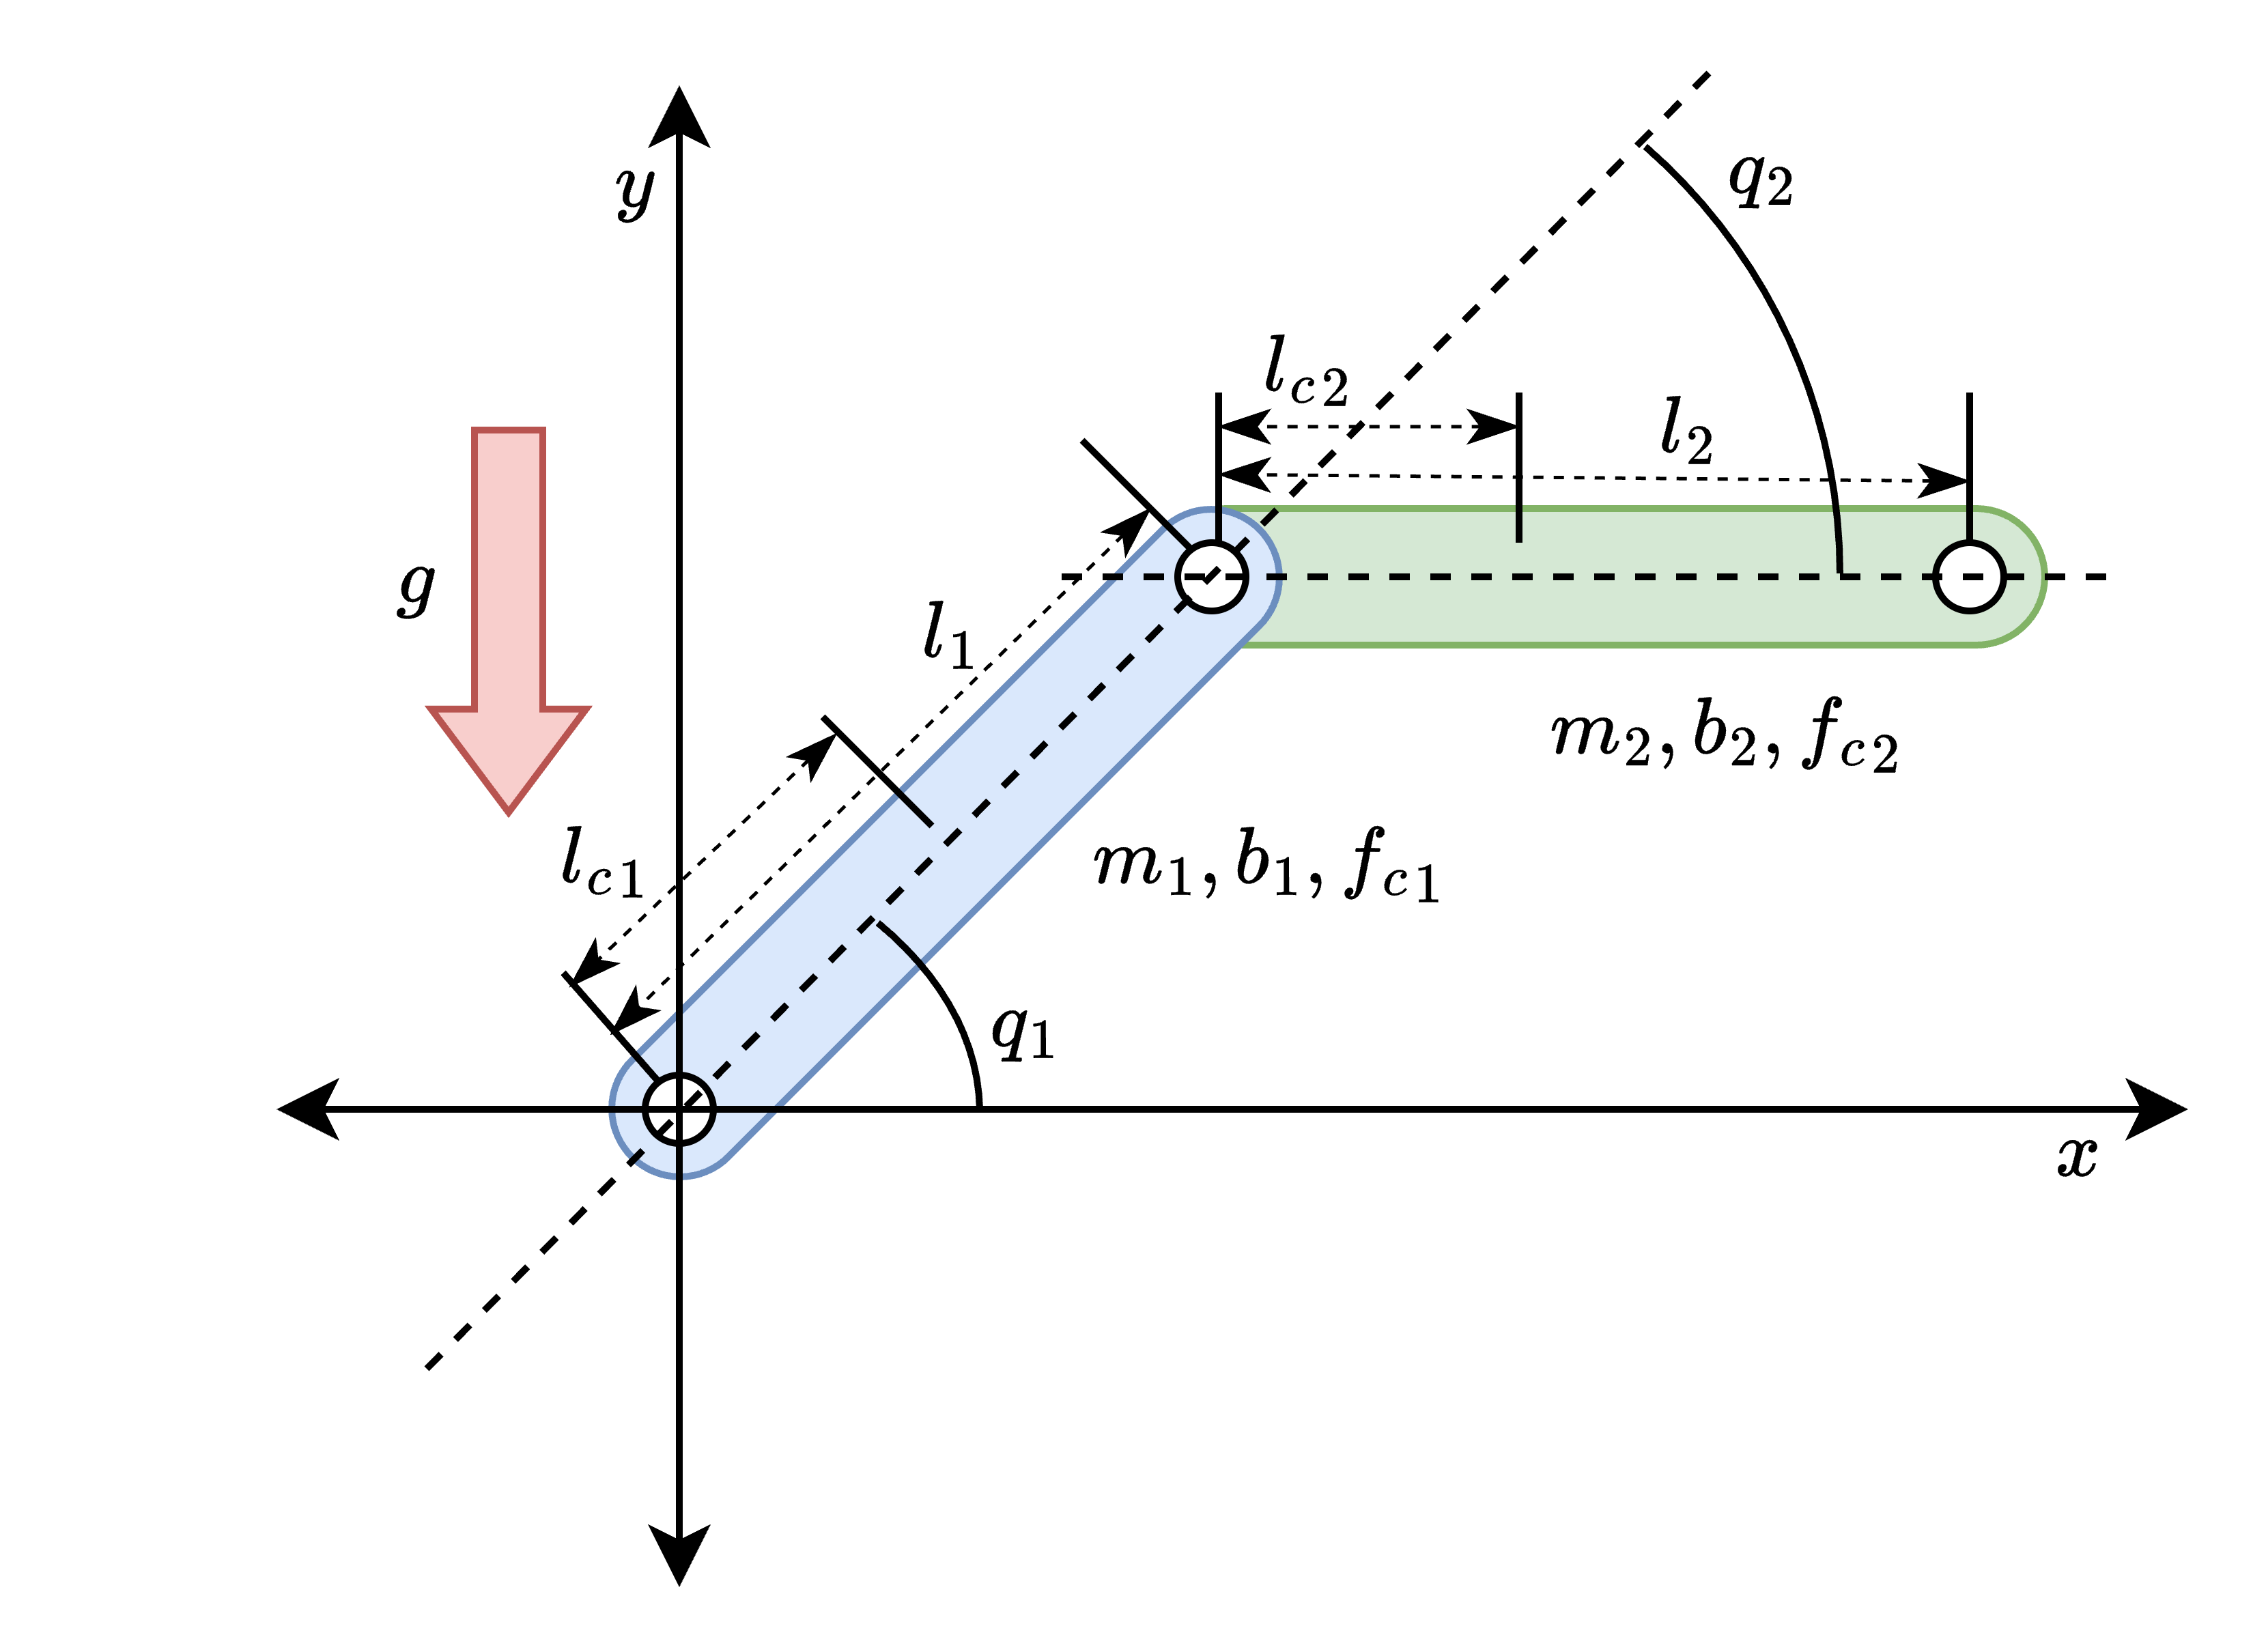
\includegraphics[width=0.7\linewidth]{RobotModel.drawio.png}
    \caption{Two-link manipulator model.}
    \label{fig: manipulator}
\end{figure}

\begin{table}[!t]
    \renewcommand{\arraystretch}{1.3}
    \caption{Controller Parameters.}
    \label{table: error norm}
    \centering
    \begin{tabular}{|c||c|c|c|c|}
    \hline
    & \textbf{link 1} & \textbf{link 2} & \textbf{Unit} & \textbf{Description} \\
    \hline 
    $m$     & 23.902 & 3.88 & kg & Mass of link\\
    \hline
    $l$     & 0.45 & 0.45 & m & Length of link\\
    \hline
    $l_c$   & 0.091 & 0.048 &m & COM of link\\
    \hline
    $b$     &  2.288 & 0.172 & Nms & Viscous coefficient\\
    \hline
    $f_c$   &  7.17 & 1.734 & Nm & Friction coefficient\\
    \hline
    \end{tabular}
    \label{table: system parameters}
\end{table}

\begin{figure}[!t]
    \centering
    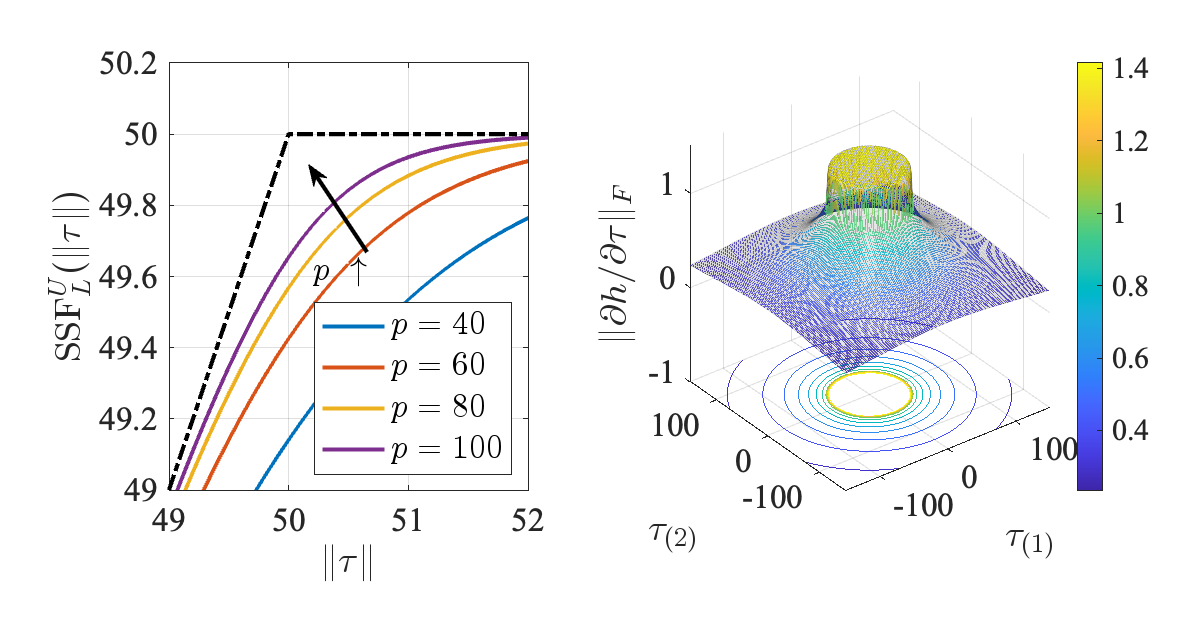
\includegraphics[width=0.9\linewidth]{fig13.eps}
    \caption{Control input saturation function.}
    \label{fig: h func}
\end{figure}

% SYSTEM FIGURE AND TABLE
% **********************************************************


Four controllers were examined for a comparative study: backstepping controller (named CM1) as a baseline; DNN-based backstepping controller (named CM2) as a existing comparative method for neuro-adaptive control; CM2 with the auxiliary system (named CM3); and the proposed controller with the maximum weight and control input ball constraints presented in Appendix \ref{sec:cstr candidates}, included (named CoNAC).

% \begin{table}[!t]
%     \renewcommand{\arraystretch}{1.3}
%     \caption{Common Parameters of Selected Controllers.}
%     \label{table: error norm}
%     \centering
%     \begin{tabular}{|c||c|c|c|c|c|c|}
%     \hline
%     & $\alpha$ & $k_1$& $k_2$ & $M_0$ & $C_0$ & $G_0$ \\
%     \hline 
%     CM1 & - & 2 & 10 & $I_2$ & $I_2$ & $0_{2\times1}$\\
%     \hline
%     CM2 & 1e3 & 2 & 10 & $I_2$ & $I_2$ & $0_{2\times1}$\\
%     \hline
%     CM3 & 1e3 & 2 & 10 & $I_2$ & $I_2$ & $0_{2\times1}$\\
%     \hline
%     C & 1e3 & 2 & 10 & $I_2$ & - & -\\
%     \hline
%     \end{tabular}
%     \label{table: control parameters}
% \end{table}

% **** CM1,2 control law *****
CM1 used the control law defined in \eqref{eq. desired control} with $\hat f=[0,0]^T$.
%CM1 has the following control gains and design parameters: $k_s=5,k_2=5, M_0=I_2, C_0=I_2, G_0=[0,0]^T  $.
% Since CM1 does not consider the unknown term, $\hat f$ was set to $[0,0]^T$. 
The control law of CM2 is same as CM1, but the unknown term is approximated by the NN i.e., $\hat f\approx \hat\Phi$.
The adaptation law of CM2 is presented in \cite{RN16}, was defined by $\dot {\hat\theta}= \text{Proj}_{\Omega}[\alpha  \nabla\hat\Phi^TM_0^{-1}e_2]$, where $\text{Proj}_{\Omega}(\cdot)$ is the projection operator \cite[Appendix E, eq.~(E.4)]{RN20} which projects an input vector to a convex set $\Omega$. The convex set was defined as ${\Omega}\triangleq \{\Omega_0 \cap\cdots\cap \Omega_k\}$, where $\Omega_i\triangleq \{\hat\theta_i\ \vert \ c_{b_i}\le 0\}, \ \forall i\in[0,\cdots, k]$ for a fair comparison with CoNAC. This convex set was the same as the maximum weight ball constraint of CoNAC.
% The maximum control input ball constraint is not addressed since the stability analysis of \cite{RN16} uses the property that  $\text{Proj}_\Omega(\cdot)$ projects to the convex set, (i.e., the constraints are generally non-convex on the $\hat\theta$-space.).
% **** CM3 control law *****
The control law of CM3 is the same as CM2, but the auxiliary system is constructed to compensate the effect of the control input saturaion.
Since the existing auxiliary systems consider the saturations of each control input, considering $h(\cdot)$, saturated control input is defined as $s(\tau)\triangleq \min(\max(\tau,-\bar\tau_s),\bar\tau_s)$, where $\bar\tau_s$ is $(\bar\tau/\sqrt{2}+\bar\tau)/2$; see Fig.~\ref{fig: ball control}.
Then the auxiliary system is defined as $\dot\zeta = A_\zeta \zeta + B_\zeta \Delta\tau,\quad \zeta\vert_{t=0} = 0$, where $\zeta\in\mathbb{R}^n$ denotes the auxiliary states, $A_\zeta=-[20,0;0;20],B_\zeta=[10,0;0,10]$ and $\Delta\tau\triangleq s(\tau)-\tau$.
The auxiliary state variables are used in the adaptation law by substituting $e_2$ with $e_2+\zeta$.
% **** CoNAC control law *****
CoNAC approximated the control law directly using the NN as defined in \eqref{eq. approximated control}.
The update rates of the multipliers were selected $\beta_{j}=0.1$.
The weight matrix $W$ was selected as $W=\text{diag}([5,1,15,15])]$.

For the NNs in the CM2, CM3 and CoNAC, the neural network input vector $q_N$ for them was selected as the desired trajectory for $x_1$ (i.e., $q_N=[r_1^T,1]^T$). 
Their DNN architectures had two hidden layers with eight nodes (i.e., $k=2, l_0=2, l_1=8, l_2=8, l_3=2$), and were assigned the same adaptation gain as $\alpha =1e3$.
Their constraint parameters were selected as $\bar\theta_0=20, \bar\theta_1=30, \bar\theta_2=50$ and $\bar\tau$ is selected as the same with the \eqref{eq. h func}. (i.e., $\bar\tau=50$)
The other parameters for CM1 to CoNAC were selected as $k_1=1.1,k_2=10,M_0=I_2,C_0=I_2,G_0=[0,0]^T$.
% The same values were assigned across all the controllers for the common parameters for a fair comparison.
% The other parameters for CM1 to CoNAC were selected as listed in Table.~\ref{table: control parameters}. The same values were assigned across all the controllers for the common parameters for a fair comparison.

% **********************************************************
% SIMULATION FIGURES
\begin{figure*}[!t]
    \centering
        \subfloat[Tracking result of CM1]{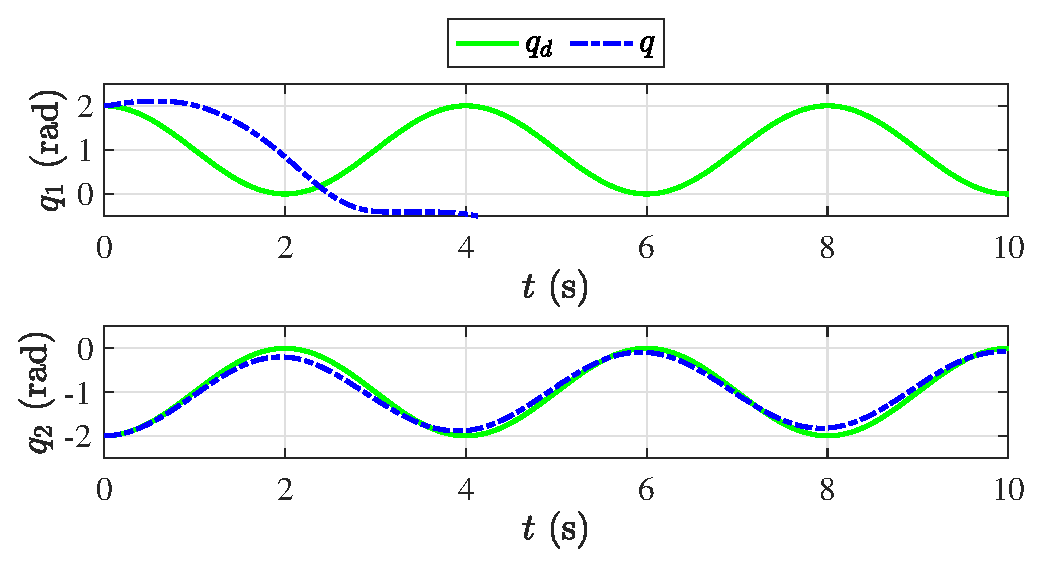
\includegraphics[width=0.45\linewidth]{fig1.eps}%
        \label{fig: tracking_CM1}}
    \qquad
        \subfloat[Tracking result of CM2]{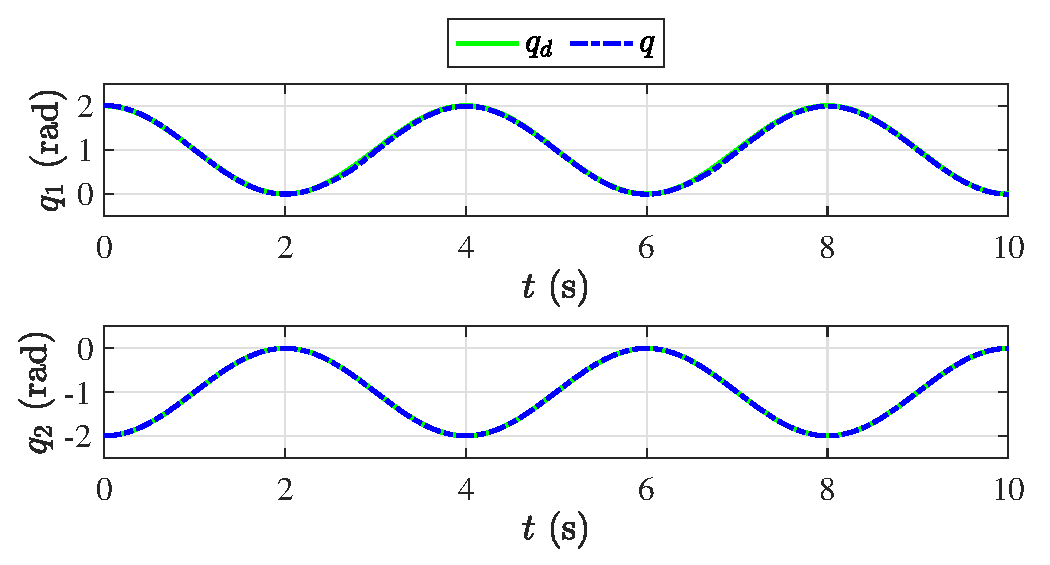
\includegraphics[width=0.45\linewidth]{fig2.eps}%
        \label{fig: tracking_CM2}}
    \vfill
        \subfloat[Tracking result of CM3]{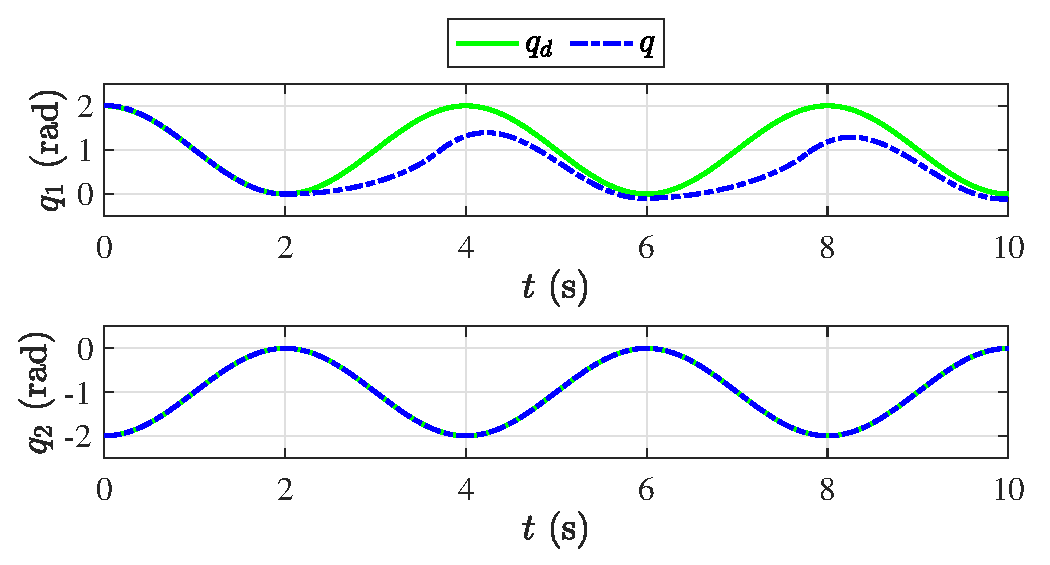
\includegraphics[width=0.45\linewidth]{fig3.eps}%
        \label{fig: tracking_CM3}}
    \qquad
        \subfloat[Tracking result of CoNAC]{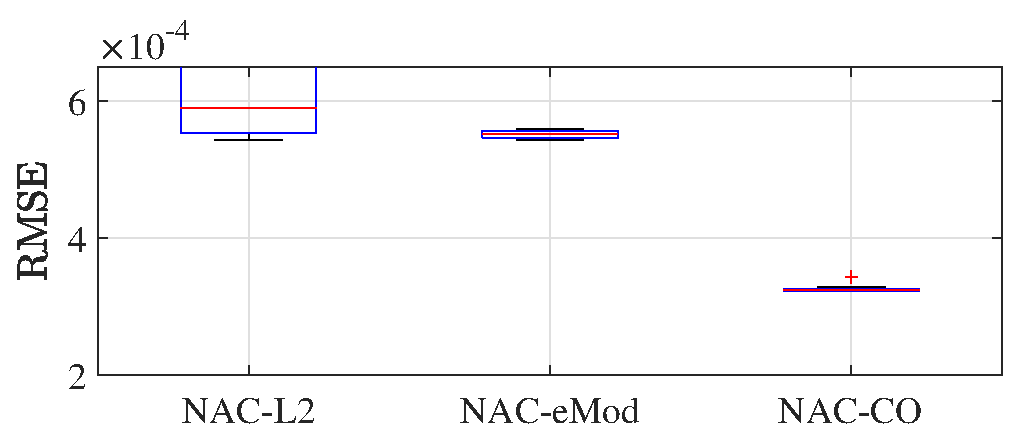
\includegraphics[width=0.45\linewidth]{fig4.eps}%
        \label{fig: tracking_CoNAC}}
    \caption{Tracking results of the selected controllers.}
    \label{fig: tracking}
\end{figure*}

\begin{figure*}[!t]
    \centering
        \subfloat[Control inputs of CM1]{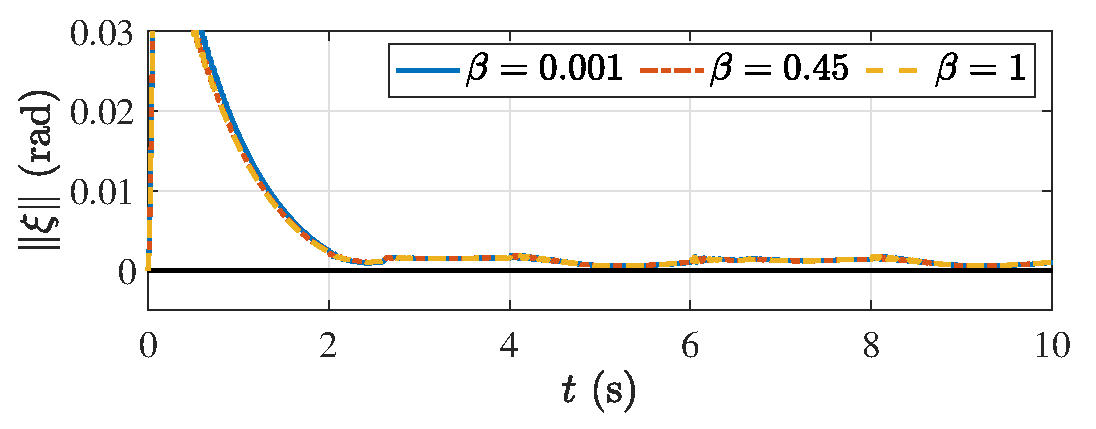
\includegraphics[width=0.45\linewidth]{fig5.eps}%
        \label{fig: control_CM1}}
    \qquad
        \subfloat[Control inputs of CM2]{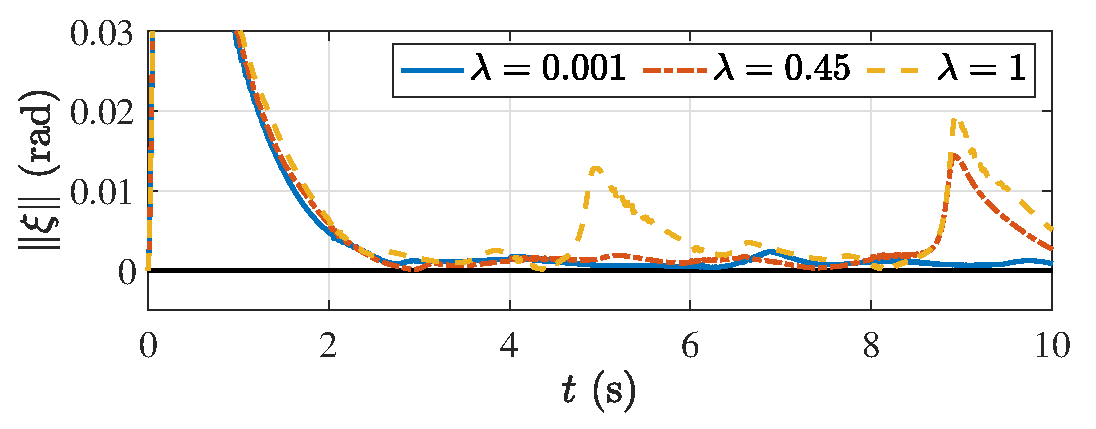
\includegraphics[width=0.45\linewidth]{fig6.eps}%
        \label{fig: control_CM2}}
    \vfill
        \subfloat[Control inputs of CM3]{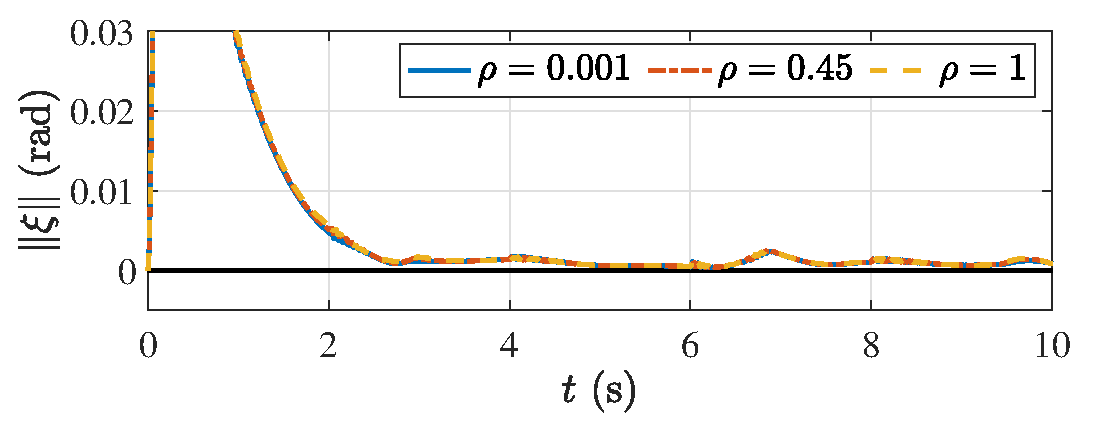
\includegraphics[width=0.45\linewidth]{fig7.eps}%
        \label{fig: control_CM3}}
    \qquad
        \subfloat[Control inputs of CoNAC]{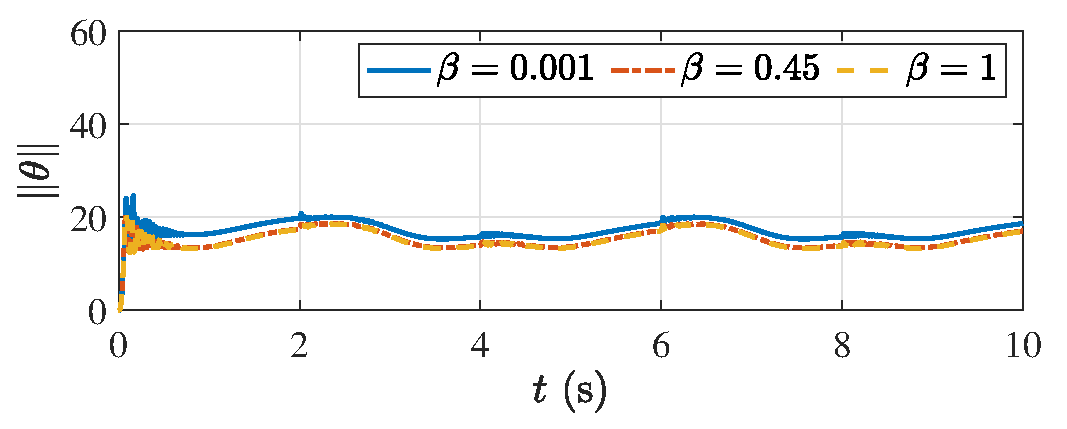
\includegraphics[width=0.45\linewidth]{fig8.eps}%
        \label{fig: control_CoNAC}}
    \caption{Produced and Saturated control inputs of the selected controllers.}
    \label{fig: control}
\end{figure*}

\begin{figure}[!t]
    \centering
    {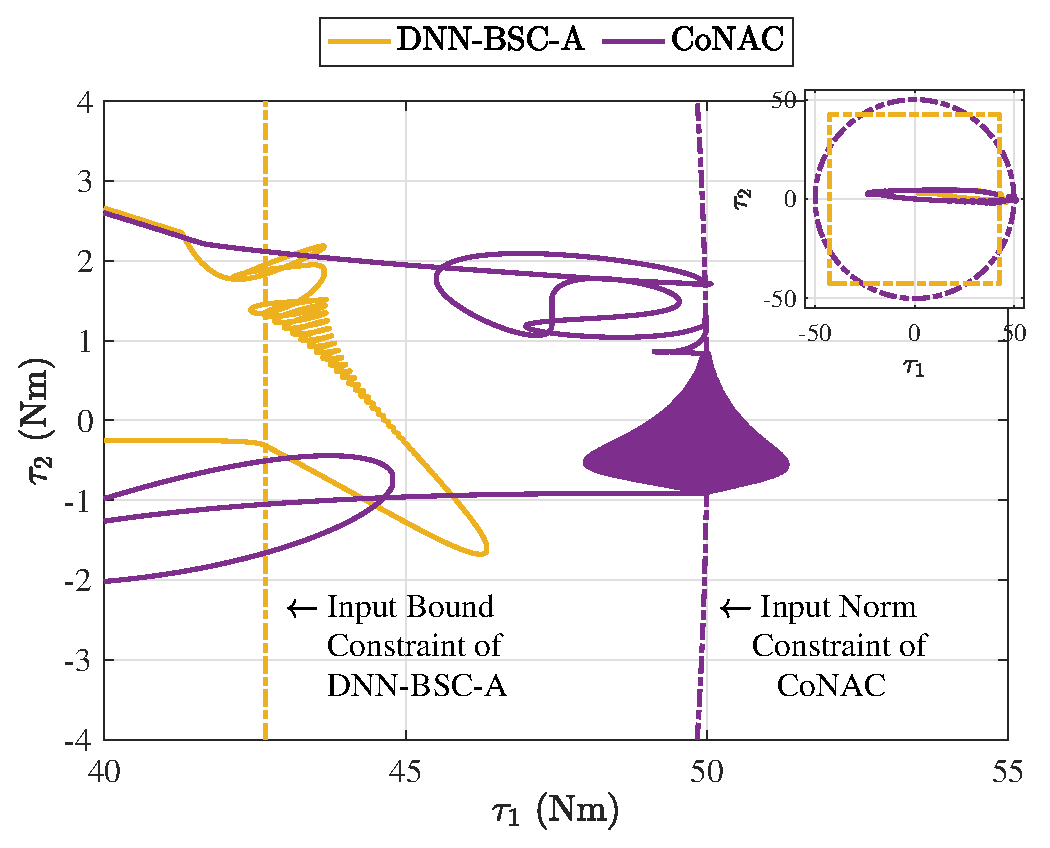
\includegraphics[width=0.9\linewidth]{fig16.eps}
    \caption{Control inputs during time interval 5s to 8s.}
    \label{fig: ball control}}
\end{figure}

\begin{figure*}[!t]
    \centering
        \subfloat[Multipliers of CoNAC]{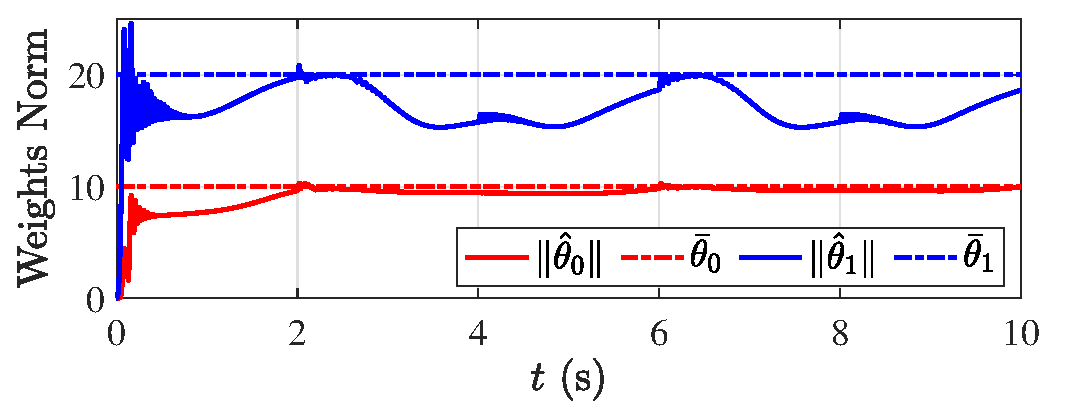
\includegraphics[width=0.45\linewidth]{fig12.eps}%
        \label{fig: multiplier_CoNAC}}
    \qquad
        \subfloat[Weight norms of CM2]{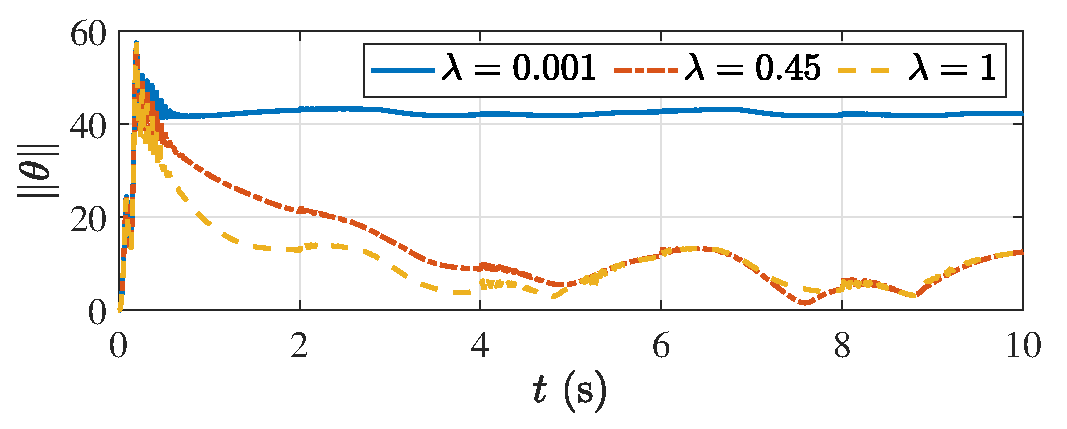
\includegraphics[width=0.45\linewidth]{fig9.eps}%
        \label{fig: weight_CM2}}
    \vfill
        \subfloat[Weight norms of CM3]{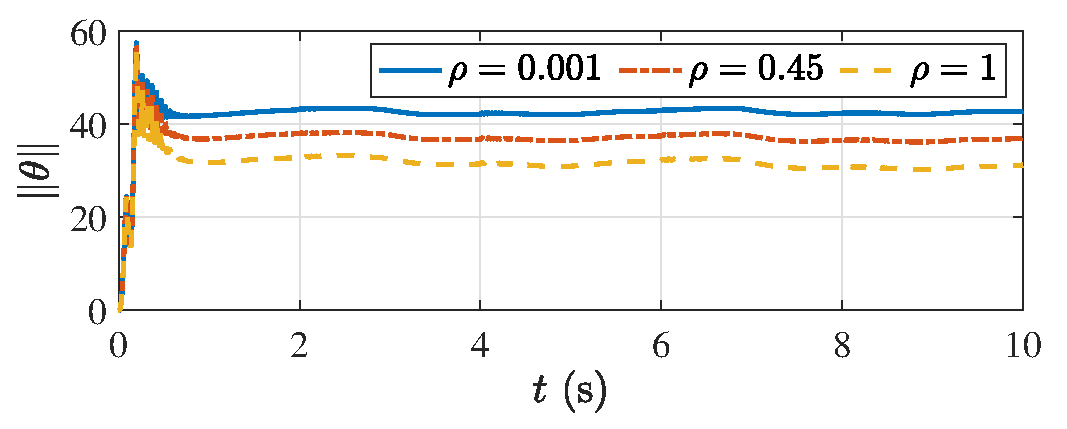
\includegraphics[width=0.45\linewidth]{fig10.eps}%
        \label{fig: weight_CM3}}
    \qquad
        \subfloat[Weight norms of CoNAC]{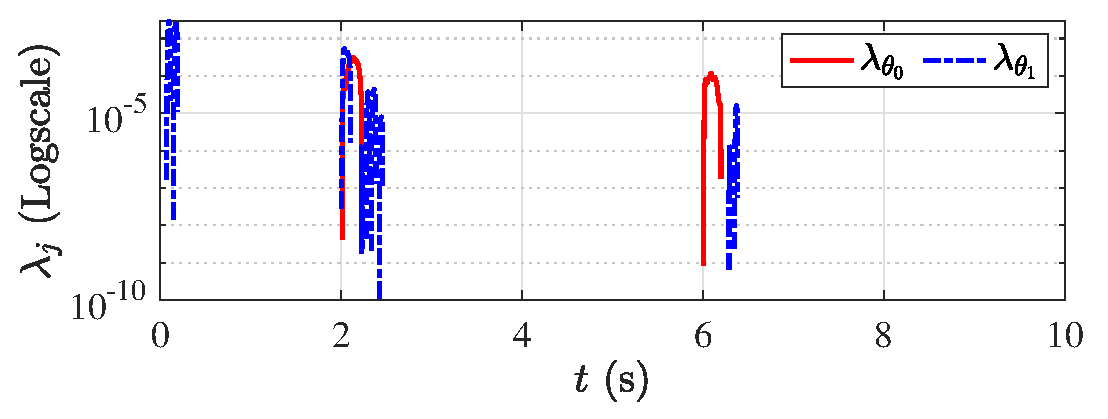
\includegraphics[width=0.45\linewidth]{fig11.eps}%
        \label{fig: weight_CoNAC}}       
    \caption{Lagrange multipliers and Weight norms of the selected controllers.}
    \label{fig: weight and multiplier}
\end{figure*}
% SIMULATION FIGURES
% **********************************************************

\subsection{Effectiveness of Neural Networks}

The tracking results of the selected controllers are shown in Fig.~\ref{fig: tracking}.
To demonstrate the effectiveness of the NNs in the BSC, $k_1$ and $k_2$ were selected as small values so that CM1 has poor performance and sufficiently large values to satisfy \eqref{eq. ctrl stable condition}.
Since the parameters of CM1 are poorly tuned, the tracking performance of CM1 in Fig.~\ref{fig: tracking_CM1} is low.
By utilizing the NNs in the BSC to compensate the uncertain terms, the tracking performances of CM2 and CM3 in Fig.~\ref{fig: tracking_CM2} and Fig.~\ref{fig: tracking_CM3} are improved.
By compensating the uncertain terms the control input of CM2 in Fig.~\ref{fig: control_CM2} is saturated.

On the other hand, CoNAC which directly approximates the control law also compensated the uncertain terms with improved performance than CM1 as shown in Fig.~\ref{fig: tracking_CoNAC}.

\subsection{Test of the Constraint Satisfactions}

As depicted in Fig.~\ref{fig: weight_CM2}-\ref{fig: weight_CoNAC}, the weight norms are bounded in the imposed maximum weight ball constraint.
In the case of CM2 which does not consider the control input constraint, the weight norm of the last layer reaches the maximum weight norm value, when the control is saturated.
It is because the weights get increased to produce larger control input to reduce the tracking error of $q_2$. (i.e., the maximum magnitude of the control input depends on the weight norm of the last layer, since the activation function is bounded.)
However, CM3 and CoNAC does not reach to the maximum weight norm, when the control saturaion occurs, since CM3 reduces the control input to regulate $\zeta$ and CoNAC adjusts the gradient of the weights using the corresponding generated multipliers as shwon in Fig.~\ref{fig: multiplier_CoNAC}.
Note that the weight norm of CoNAC reaches the maximum weight norm in the first control cycle due to the initial approximation error of the weights.
Besides, the overall weight norm of CoNAC is larger than CM2 and CM3, since there is no conventional controller in CoNAC.

In the case of control saturation constraint, as shown in Fig.~\ref{fig: control_CM3} and Fig.~\ref{fig: control_CoNAC}, the auxiliary system of CM3 and the proposed weight optimizer of CoNAC reduced the saturation of the control input.
However, the performance of CM3 is lower than CM2 and CoNAC, since the auxiliary handles the saturation of each control input. (i.e., the feasible control input set can be represented as a rectangle in $\tau$-space as shown in Fig.~\ref{fig: ball control}.)
By comparison, CoNAC can produce the physically maximum control input with the improved tracking performance, since it can satisfy the nonlinear control constraint. 

Futhermore, as shown in Fig.~\ref{fig: ball control}, the control input trajectory of CMe depends on the dynamics characteristics of the auxiliary system.
The control input constraint is satisfied when the $\zeta$ is generated enough to compensate the control input saturation.
However, CoNAC can satisfy the constraint without the effect of certain dynamics, since the corresponding multiplier generated as the constraint is violated.

Meanwhile, CM2 and CM3 is based on BSC, and the desired controller $\tau^*$ of CoNAC is based on the BSC which may produce larger control input by canceling the stabilizing system dynamics.
Therefore, CM2, CM3, and CoNAC produced the saturated control input.
These control results show why the control saturation should be handled.

In Fig.~\ref{fig: weight_CoNAC}, it is shown that the norm of the weights is constant when the constraints are in the active set.
It means that the KKT condition is satisfied such that $d{\hat\theta}/dt=-\alpha\partial L/\partial \hat\theta=0$ (i.e., $\partial J/\partial\hat\theta = \sum_{j\in\mathcal {A}}\lambda_j\nabla_{\hat\theta} c_j)$, by the multipliers increased due to the violation of the constraints as shown in Fig.~\ref{fig: multiplier_CoNAC}.
Because the simulation is implemented in a digital computer, the multipliers repeat to disappear and be generated, since the constraints are satisfied and violated in the digital process.

\subsection{Analysis of the Neural Network}

Generally, the existing literature states that the maximum norms of the weights should be sufficiently large (i.e., $\bar\theta_i \gg 0$) since the designer does not know where the global optimal point of the weights is.
However, using the physical prior knowledge of the system, one can guess the proper value of the maximum norm, since the magnitude of the control input depends on the last layer's weights due to the bounded activation function.
Furthermore, the simulation study shows that the selected controllers have sufficiently good performances with the small maximum weight norms.
It means that the local optimal point of the weights are more effective for the stability analysis and the limitating the control input's amplitude.

Since it is generally known that the deeper NNs have better approximation performance with less computation cost, the NNs should have more layers.
However, because the NNs in this paper utilize $\tanh(\cdot)$ as the activation function, the NNs have the gradient vanishing problem as shown in Fig.~\ref{fig: weight_CM2}-\ref{fig: weight_CoNAC}. (i.e., the weight updates are smaller as its layer is closer to the input layer.)
To address this issue, the activation function should be selected as the ReLU or the Leaky ReLU, while ensuring the stability of the controller.

%  SECTION CONCLUSION ======================================
\section{Conclusion}\label{sec:conclusion}

In this paper, the contstrained optimization-baesd neuro-adaptive controller for the uncertain Euler-Lagrange system was proposed.
The stability of the controller was analyzed by the Lyapunov stability analysis and the candidates of the constraints of the control input are introduced.
The effectiveness of the proposed controller was validated by the simulation, and demonstrated that the proposed controller can address the constraints while maintaining the tracking performance and satisfying the KKT condition.
In the future, we will study the neuro-adaptive controller which can address the constraints of the states using the constrained optimization approach.

%  SECTION APPENDIX ======================================
 \appendices

 \section{Candidates of Constraints}\label{sec:cstr candidates} 

This section introduces common constraints of the control input saturation used in neuro-adaptive control. The proposed controller can incorporate any combination of the following candidates, provided they satisfy the Assumption \ref{assum1}, \ref{assum2}. 

\subsection{Maximum Weight Ball}\label{sec:cstr weight ball}

The inequality constraint $\mathbf{c}_{b}\triangleq [c_{b_i}]_{i\in[0,\cdots ,k]}\in\mathbb R^{k+1}$ limits the maximum norm of each layer's weight matrix, where
\begin{equation*}
    c_{b_i}=\Vert \hat\theta_i\Vert^2 -\bar\theta_i^2 \le 0
    \label{eq. cstr weight ball}
\end{equation*}
with $\bar\theta_i<\infty$ denoting the maximum norm of $\hat\theta_i$.
The gradient of $\mathbf{c}_b$ with respect to $\hat\theta$ is given by
\begin{equation*}
    \nabla \mathbf c_b 
    \triangleq
    \begin{bmatrix}
        \nabla  c_{b_0}^T
        \\ 
        \vdots 
        \\
        \nabla  c_{b_k}^T
    \end{bmatrix}
    = 2\cdot 
    \begin{bmatrix}
        0&0&\cdots & \hat\theta_0^T\\
        \vdots&\vdots&\ddots&\vdots\\
        0&\hat\theta^T_{k-1}&\cdots &0\\
        \hat\theta^T_k&0&\cdots &0
    \end{bmatrix}
    \in\mathbb R^{k+1\times\Xi}
\end{equation*}
where $\nabla c_{b_i}\triangleq \partial c_{b_i}/\partial \hat\theta$ for all $i \in \left[0,\cdots,k\right]$.

\begin{remark} Imposing the maximum weight ball constraint is analogous to applying $L_2$-regularization, a common technique used in DNN training to prevent parameter drift or overfitting \cite{RN23}, by minimizing the $L_2$ norm of the trainable weights $\hat\theta$. Typically, $L_2$-regularization adds a term $\lambda\Vert\hat\theta\Vert_2^2$ to the objective function $J$, where $\lambda\in\mathbb R_{>0}$ is a constant $L_2$ coefficient. This term biases the trainable weights $\hat\theta$ toward the origin (i.e., $\hat\theta = 0$) in the adaptation law \eqref{eq. adaptation law th}. In contrast, within the proposed controller, the term associated with the maximum weight ball constraint in the adaptation law (i.e., $\sum_{j\in\mathcal{A}}\lambda_j \nabla c_j$ in \eqref{eq. adaptation law th}) vanishes when the constraint is satisfied (i.e., $\lambda_j = 0$).
    % 1. 제약조건이 사라져 자유롭게 ball condition 내에서 optimal point로 접근할 수 있다.
    As a result, $\hat\theta$ can still converge to $\theta^*$ without being restricted to the origin.
    Moreover, $\lambda_{b_i}$ which corresponds to $\lambda$ varies as the constraint is violated, while $L_2$-regularization has a constant coefficient.
    \label{remark: ball cstr}
\end{remark}

\subsection{Control Input Saturaion}

Most physical systems have control input saturation due to their electrical and mechanical limitations, expressed as $\mathbf{c}_{M}\triangleq [c_{M_i}]_{i\in[1,\cdots,n]}$ and $\mathbf{c}_{m}\triangleq [c_{m_i}]_{i\in[1,\cdots,n]}$, where
\begin{equation}
    \begin{aligned}
        c_{M_i}=\tau_{(i)} - {\tau_{M_i}} \le 0
        \\
        c_{m_i}={\tau_{m_i}}-\tau_{(i)} \le 0
    \end{aligned}
    \label{eq. cstr input saturation}
\end{equation}
with $\tau_{M_i}$ and $\tau_{m_i}$ representing the maximum and minimum control input values, respectively.
% The corresponding Lagrange multipliers are $\lambda_{u_j,i},\ \forall j\in[M,m]$. 
The gradients of $\mathbf{c}_{M}$ and $\mathbf{c}_{m}$ with respect to $\hat\theta$ are given by
\begin{equation}
    \begin{aligned}
        \nabla \mathbf c_{M} \triangleq
        & 
        \begin{bmatrix}
            \nabla c_{M_1}^T \\
            \vdots \\
            \nabla c_{M_n}^T \\
        \end{bmatrix}
         = -\nabla \hat\Phi
         \\
        =&
        -\begin{bmatrix}
            (I_{l_{k+1}}\otimes \phi_{k}^T)&
            % V_k^T \phi_{k}' (I_{l_{k}}\otimes  \phi_{k-1}^T)&
            \cdots &
            (
            \cdot
            )
        \end{bmatrix} 
        &
        \in
        \mathbb R^{n\times \Xi}
        , 
        \\
        \nabla \mathbf c_{m}
         \triangleq
        & 
        \begin{bmatrix}
            \nabla c_{m_1}^T \\
            \vdots \\
            \nabla c_{m_n}^T \\
        \end{bmatrix}
        = +\nabla \hat\Phi  
        \\
        =&
        +\begin{bmatrix}
            (I_{l_{k+1}}\otimes \phi_{k}^T)&
            % V_k^T \phi_{k}' (I_{l_{k}}\otimes  \phi_{k-1}^T)&
            \cdots &
            (
            \cdot
            )
        \end{bmatrix} 
        &
        \in
        \mathbb R^{n\times \Xi}
    \end{aligned}
    \label{eq. nabla input sat}
\end{equation}
where $\nabla c_{M_i}\triangleq \partial c_{M_i}/\partial \hat\theta$ and $\nabla c_{m_i}\triangleq \partial c_{m_i}/\partial \hat\theta$.

\subsection{Maximum Control Input Ball}

Consider the control input $\tau$ as the torque of each actuator corresponding to each generalized coordinate. The torque is typically linearly proportional to the current, and if the actuators share a common power source, they are subject to a total current limitation. This condition can be expressed by the following inequality constraint: $c_{u_b} \in\mathbb R$, where 
\begin{equation}
    c_{u_b}=\Vert\tau\Vert^2 -\bar\tau^2  \le 0
    \label{eq. cstr input ball}
\end{equation}
with $\bar\tau\in\mathbb{R}_{>0}$ denoting the maximum allowable control input magnitude.
% The corresponding Lagrangian multipier is $\lambda_{u_b}$. 
The gradients of $c_{u_b}$ with respect to $\hat\theta$ are given by
\begin{equation}
    \nabla c_{u_b} = -\sum_{i=1}^n 2\tau_{(i)} 
    \bigg(
        \text{row}_i(-\nabla\hat\Phi)
    \bigg)^T  
    \in \mathbb R^{\Xi}.
    \label{eq. nabla input ball}
\end{equation}

Constraints \eqref{eq. cstr input saturation} and \eqref{eq. cstr input ball} cannot be imposed for the proposed controller simultaneously, because their gradients \eqref{eq. nabla input sat} and \eqref{eq. nabla input ball} are linearly dependent and accordingly violate the LICQ condition.

\section{Proof of Lemma \ref{lem1}}\label{sec:proof lem1}

\begin{figure}[!t]
    \centering
    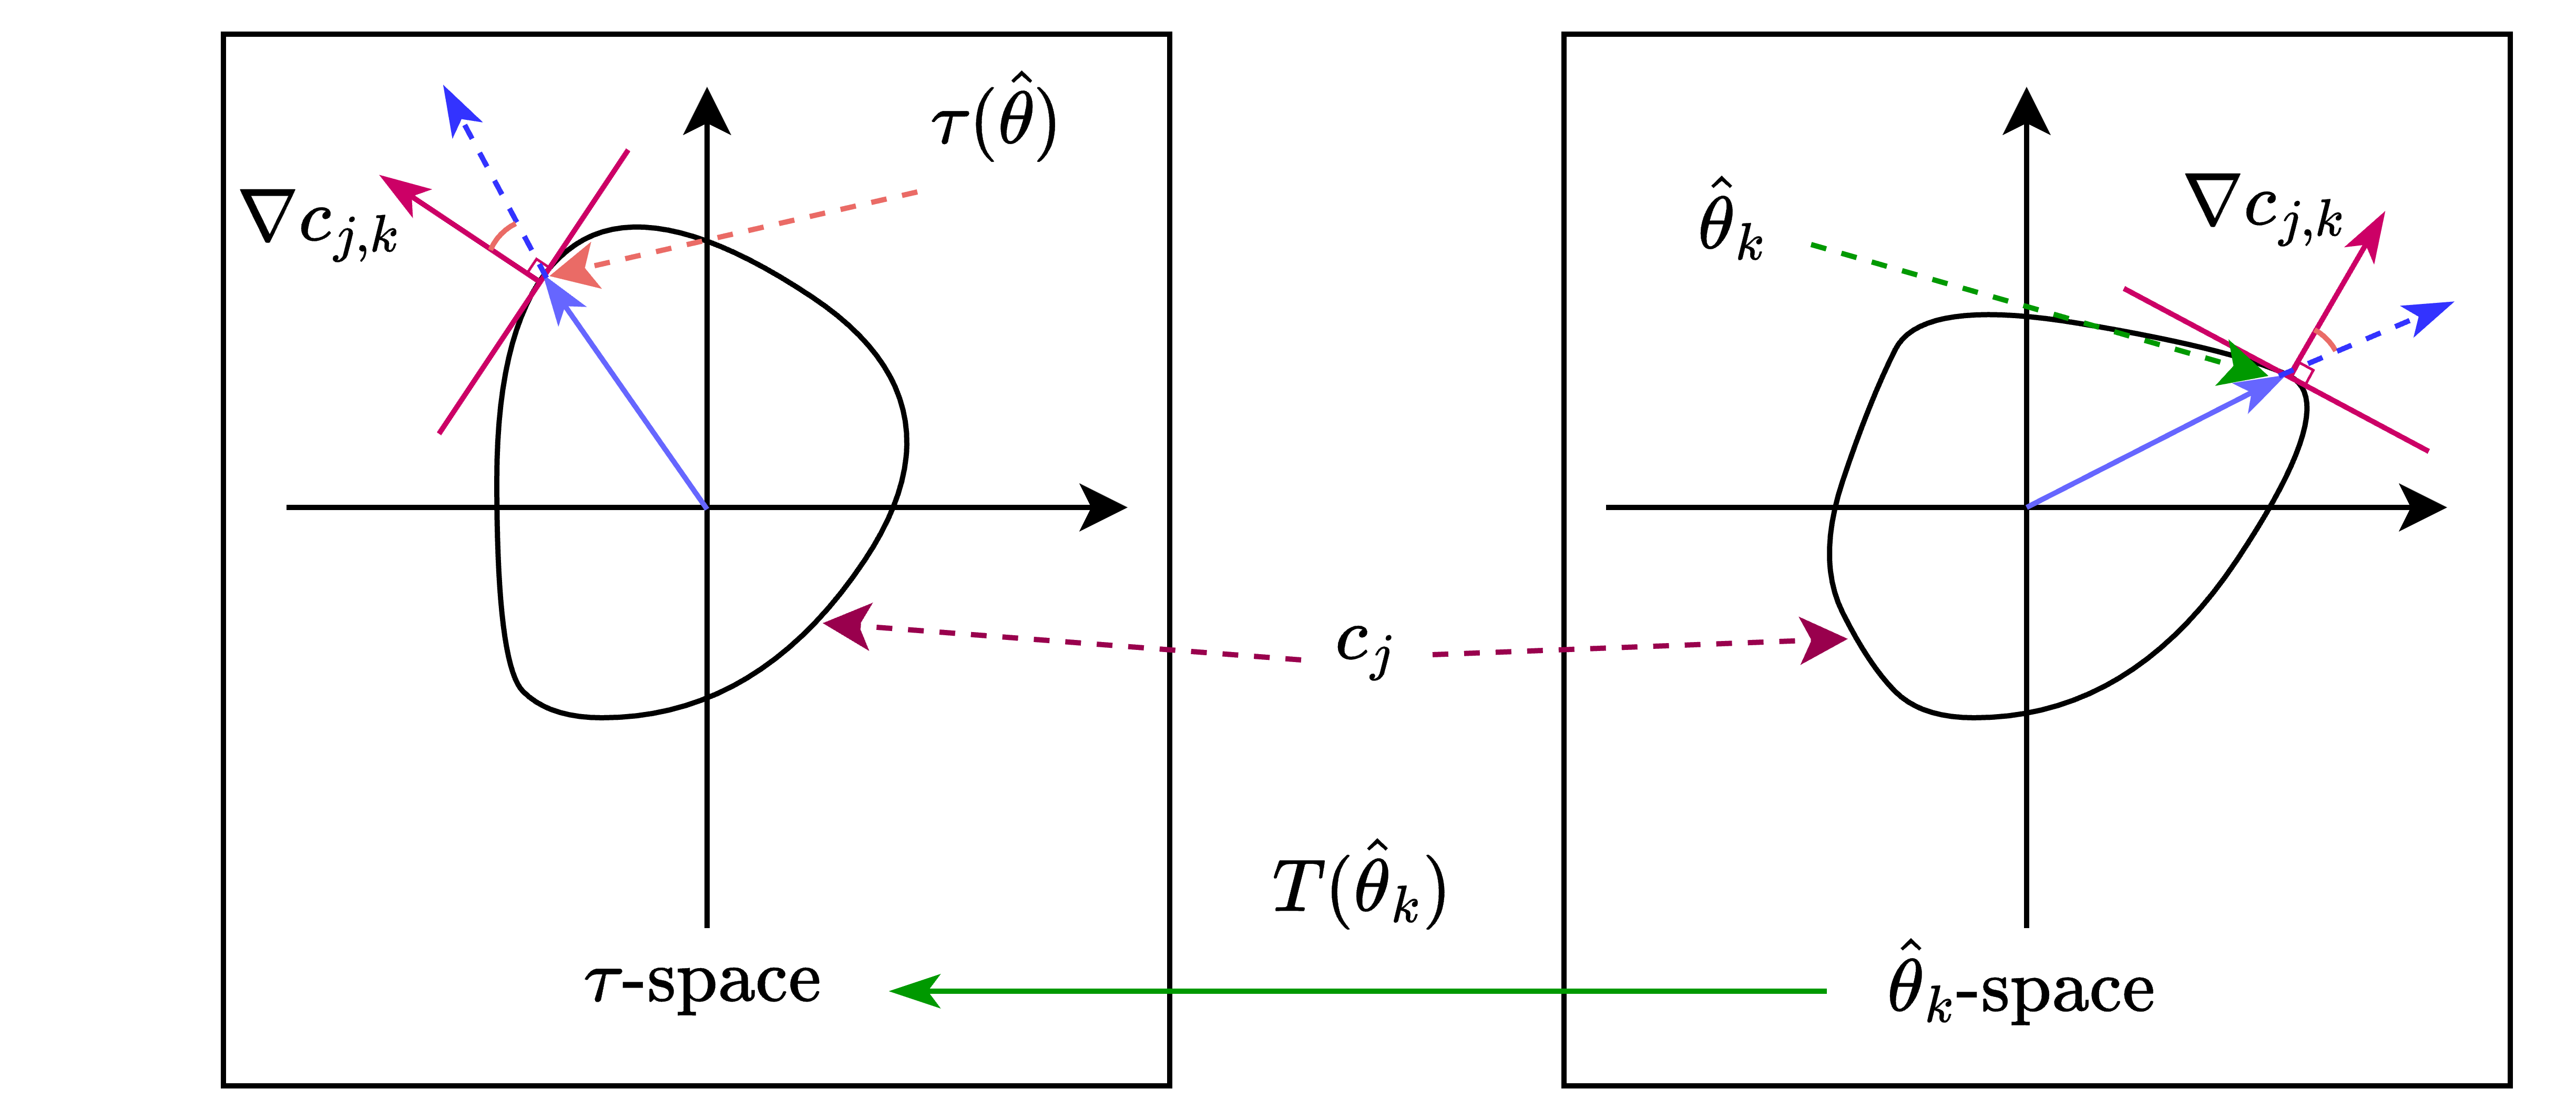
\includegraphics[width=1.1\linewidth]{spaces.drawio.png}
    \caption{Convexity of the constraints.}
    \label{fig: spaces}
\end{figure}

From the definition of the control input, a linear map $T(\cdot):\hat\theta_k\to\tau$ can be obtained such that 
\begin{equation}
    \tau = -\hat\Phi = -\hat V_k \hat\phi_k = -(I\otimes \hat\phi_k^T)\hat\theta_k = T(\hat\phi_k) \hat\theta_k.
\end{equation}
Therefore, the convexity of the constraints in the $\tau$-space holds in the $\hat\theta_k$-space, as depicted in Fig.~\ref{fig: spaces}, i.e., $\nabla c_{j,k}^T\hat\theta_k>0$.

Let $\omega^*\triangleq [\theta_k^{*T}; [\hat\theta_i]_{i\in[0,\cdots,k-1]}]$ and $\hat\omega\triangleq [\hat\theta_k^{T}; [\hat\theta_i]_{i\in[0,\cdots,k-1]}]$. 
If the Assumption \ref{assum1} is satisfied (i.e., $c(\omega^*)<0,c(\hat\omega)\ge 0$), $\nabla c_{j,k}^T\hat\theta_k>0$ also implies $\nabla c_{j,k}^T\tilde\theta_k>0$ such that 
\begin{equation}
    \begin{aligned}
        -\nabla c_{j,k}^T \tilde\theta_k=&\nabla c_{j,k}^T(\theta_k^*-\hat\theta_k)
        =
        {d\over d\delta } c_j(\hat\omega +\delta (\omega^*-\hat\omega))\bigg\vert _{\delta=0} \\
        =& \lim_{\delta\to 0} {c_j(\hat\theta-\delta(\omega^*-\hat\omega)) + c_j(\hat\omega)\over \delta}\\
        \le& \lim_{\delta\to0} {\delta c_j(\omega^*) + (1-\delta) c_j(\hat\omega)-c_j(\hat\omega)\over \delta}
        \\
        =& c_j(\omega^*) - c_j(\hat\omega) < 0
        \end{aligned}
\end{equation}

One can easily prove that $\nabla c_{j,k}^T\hat\theta_k>0$ holds for all introduced constraints in Appendix \ref{sec:cstr candidates}.

% \section{Details of CM3}\label{sec:detail CM3}

% As motivated by 
% \color{red}
% \cite{RN111}-\cite{RN110}
% \color{black}
% , the auxiliary system is introduced to compensate the control input saturation, as
% \begin{equation}
%     \dot \zeta  = 
%     \begin{cases}
%         -K_\zeta \zeta - 
%         \bigg({
%         \vert e_2^TM_0^{-1}k_\zeta\Delta\tau\vert +0.5k_\zeta^2\Delta \tau^T\Delta \tau
%         \over
%         \Vert\zeta\Vert^2
%         }\bigg)
%         \zeta
%         +
%         k_\zeta
%         \Delta \tau,
%         \\
%         \quad\quad\quad
%         \quad\quad\quad
%         \quad\quad\quad
%         \quad\quad\quad
%         \quad\quad\quad\quad

%         \Vert \zeta\Vert \ge \mu
%         \\
%         -K_\zeta \zeta+ k_\zeta\Delta \tau, 
%         \quad\quad\quad
%         \quad\quad\quad
%         \quad\quad\quad\ 
%         \Vert\zeta\Vert < \mu
%     \end{cases}
%     \label{eq. aux system}
% \end{equation}
% where $\zeta$ denotes the auxiliary state variables, $\Delta\tau \triangleq h(\tau) - \tau$, $\mu\in\mathbb R_{>0}$ is a positive constant, and $K_\zeta=K_\zeta^T>0$.
% To scale the difference of the magnitude between $e_2$ and $\Delta\tau$, $k_\zeta\in\mathbb R_{>0}$ is used.

% Let the control law be defined as 
% \begin{equation}
%     \tau =-k_2M_0e_2-M_0K_p \zeta -M_0e_1+C_0x_2+G_0-\hat f+M_0 \dot r_2
%     \label{eq: control law CM3}
% \end{equation}
% where $K_p$ denotes the gain matrix.
% Then the system is bounded with the following criteria: $k_1 > 0, k_2 >1/2, k_\zeta>1, \mu>1, K_p > 0, K_\zeta >{1\over 2}(K_p^TK_p+I),\dot{\hat\theta } = \text{Proj}_{\Omega}[\alpha\nabla\hat\Phi^T{M^{-1}}^{T} e_2]$.
% The proof of the boundedness can be readily obtained using the Lyapunov function $V=(1/2)e_1^Te_1+(1/2)e_2^Te_2+(1/2\alpha)\tilde\theta^T\tilde\theta + (1/2)\zeta^T\zeta$.

%  BIBLIOGRAPHY ============================================
\bibliographystyle{ieeetr}
\bibliography{refs}

% \begin{IEEEbiographynophoto}{Myeongseok Ryu}
% \lipsum[1]
% \end{IEEEbiographynophoto}

\begin{IEEEbiography}[{\includegraphics[width=1in,height=1.25in,clip,keepaspectratio]{MRyu.jpg}}]{Myeongseok Ryu}
recieved B.S. degree in Mechanical Engineering from Incheon National University, in 2023. In 2023 he is persuing M.S. degree in the School of Mechanical and Robotics Engineering at GIST. His research interests include adaptive control, neural network control, optimization, and reinforcement learning.
\end{IEEEbiography}

\begin{IEEEbiography}[{\includegraphics[width=1in,height=1.25in,clip,keepaspectratio]{HDong.jpeg}}]{Donghwa Hong}
received B.S. degree in Physics and Engineering Physics from Yonsei University, in 2023. In 2023 he is persuing M.S. degree in the School of Mechanical and Robotics Engineering at GIST. His research interests include impedance control, human interactive control, adaptive control, and neural network control.  
\end{IEEEbiography}

\begin{IEEEbiography}[{\includegraphics[width=1in,height=1.25in,clip,keepaspectratio]{KChoi.jpg}}]{Kyunghwan Choi}
received B.S., M.S., and Ph.D. degrees in Mechanical Engineering from KAIST, Daejeon, South Korea, in 2014, 2016, and 2020, respectively. He then worked at the Center for Eco-Friendly \& Smart Vehicles at KAIST as a Postdoctoral Fellow and a Research Assistant Professor. He is currently an Assistant Professor in the School of Mechanical and Robotics Engineering at GIST, where he directs the Mobility Intelligence and Control Laboratory. His research focuses on optimal control for mobility systems.
\end{IEEEbiography}

\end{document}
